% do not change these two lines (this is a hard requirement
% there is one exception: you might replace oneside by twoside in case you deliver 
% the printed version in the accordant format
\documentclass[11pt,titlepage,oneside,openany]{book}
\usepackage{times}
\usepackage{eso-pic} % used by \AddToShipoutPicture
\RequirePackage{fancyhdr}
\RequirePackage{natbib}
\usepackage{booktabs}
% modification to natbib citations
\setcitestyle{authoryear,round,citesep={;},aysep={,},yysep={;}}

\usepackage{graphicx}
\usepackage{latexsym}
\usepackage{amsmath}
\usepackage{amssymb}

\usepackage{ntheorem}

% \usepackage{paralist}
\usepackage{tabularx}
\usepackage{tablefootnote}
% this packaes are useful for nice algorithms
\usepackage{algorithm}
\usepackage{algorithmic}

% well, when your work is concerned with definitions, proposition and so on, we suggest this
% feel free to add Corrolary, Theorem or whatever you need
\newtheorem{definition}{Definition}
\newtheorem{proposition}{Proposition}
\usepackage[colorlinks = true,
            linkcolor = blue,
            urlcolor  = blue,
            citecolor = blue,
            anchorcolor = blue]{hyperref}
\usepackage{multirow}
\usepackage{array,ragged2e}
\newcolumntype{P}[1]{>{\RaggedRight\arraybackslash} p{#1}}
\newcolumntype{M}[1]{>{\RaggedRight\arraybackslash} m{#1}}
% its always useful to have some shortcuts (some are specific for algorithms
% if you do not like your formating you can change it here (instead of scanning through the whole text)
\renewcommand{\algorithmiccomment}[1]{\ensuremath{\rhd} \textit{#1}}
\def\MYCALL#1#2{{\small\textsc{#1}}(\textup{#2})}
\def\MYSET#1{\scshape{#1}}
\def\MYAND{\textbf{ and }}
\def\MYOR{\textbf{ or }}
\def\MYNOT{\textbf{ not }}
\def\MYTHROW{\textbf{ throw }}
\def\MYBREAK{\textbf{break }}
\def\MYEXCEPT#1{\scshape{#1}}
\def\MYTO{\textbf{ to }}
\def\MYNIL{\textsc{Nil}}
\def\MYUNKNOWN{ unknown }
% simple stuff (not all of this is used in this examples thesis
\def\INT{{\mathcal I}} % interpretation
\def\ONT{{\mathcal O}} % ontology
\def\SEM{{\mathcal S}} % alignment semantic
\def\ALI{{\mathcal A}} % alignment
\def\USE{{\mathcal U}} % set of unsatisfiable entities
\def\CON{{\mathcal C}} % conflict set
\def\DIA{\Delta} % diagnosis
% mups and mips
\def\MUP{{\mathcal M}} % ontology
\def\MIP{{\mathcal M}} % ontology
% distributed and local entities
\newcommand{\cc}[2]{\mathit{#1}\hspace{-1pt} \# \hspace{-1pt} \mathit{#2}}
\newcommand{\cx}[1]{\mathit{#1}}
% complex stuff
\def\MER#1#2#3#4{#1 \cup_{#3}^{#2} #4} % merged ontology
\def\MUPALL#1#2#3#4#5{\textit{MUPS}_{#1}\left(#2, #3, #4, #5\right)} % the set of all mups for some concept
\def\MIPALL#1#2{\textit{MIPS}_{#1}\left(#2\right)} % the set of all mips





\begin{document}

\pagenumbering{roman}
% lets go for the title page, something like this should be okay
\begin{titlepage}
	\vspace*{2cm}
  \begin{center}
   {\Large The Extremes of Good and Evil\\}
   \vspace{2cm} 
   {Master Thesis\\}
   \vspace{2cm}
   {presented by\\
    Earl Hickey \\
    Matriculation Number 9083894\\
   }
   \vspace{1cm} 
   {submitted to the\\
    Data and Web Science Group\\
    Prof.\ Dr.\ Right Name Here\\
    University of Mannheim\\} \vspace{2cm}
   {August 2014}
  \end{center}
\end{titlepage} 

% no lets make some add some table of contents
\tableofcontents
\newpage

\listofalgorithms

\listoffigures

\listoftables

% evntuelly you might add something like this
% \listtheorems{definition}
% \listtheorems{proposition}

\newpage


% okay, start new numbering ... here is where it really starts
\pagenumbering{arabic}

\chapter{Introduction}
\label{cha:intro}
Nowadays, most of real-world information such as social, biological information can be well encoded into graphs \citep{lu2011link}. Each vertex represents an entity, an object, or a biological element (proteins, genes, etc.), while each edge represents a relation or an interaction between entities. Those graphs can be thought of as Knowledge Graphs (KGs), and each connection between two entities is a \textit{fact}. Formally, a \textit{fact} is a tuple that contains two entities and their relation denoted as $(s,p,o)$, e.g., \textit{(Berlin, isCapitalOf, Germany)}. \textit{Berlin} is subject entity ($s$), \textit{Germany} is object entity ($o$) and their relation/predicate ($p$) is \textit{isCapitalOf}.

Unfortunately, KGs such as biological networks \citep{amaral2008truer, stumpf2008estimating, yu2008high}, contain numerous undiscovered relations between two entities. This is essential since existing knowledge graphs are often missing many facts, and some of the edges they contain are incorrect \citep{angeli2013philosophers}. 
% Therefore, several studies \citep{nickel2011three, lao2010relational, dong2014knowledge, socher2013reasoning}, have proposed different models to predict the existence of a relation between two entities.  

% There are two approaches to adding missing relation \citep{wang2017knowledge}: (1) predicting a missing entity based on a given entity and relation - \textit{entity prediction}, and (2) directly predicting the relation between two entities - \textit{relation prediction}.
In KG, adding missing relation between two entities is typically referred to as predicting an entity with a specific relation with another given entity \citep{wang2017knowledge}. This task is entity prediction \citep{lin2015modeling} and has been tested extensively in previous literature \citep{bordes2013translating, lin2015learning, nickel2016holographic, wang2014knowledge}. Besides that, directly predicting the existence of a relation between two given entities can also be used to add missing relation between two entities. That task is called relation prediction \citep{lin2015modeling, xie2016representation}. 
Formally, the difference between entity prediction and relation prediction would be the model's questions: for entity prediction, the model tries to answer $(s,p,?)$. In contrast, the relation prediction model tries to answer $(s,?,o)$. 

Most KGE models can perform both entity and relation predictions \citep{wang2017knowledge}; e.g., RESCAL \citep{nickel2011three}, TransE \citep{bordes2013translating}, ComplEx \citep{trouillon2016complex}, TuckER \citep{balazevic-etal-2019-tucker}, RotatE \citep{sun2019rotate}, and many more. However, in most KGE studies \citep{yang2014embedding, wang2014knowledge, trouillon2016complex, shang2018endtoend, sun2019rotate}, entity prediction is the main task for training, comparing, and testing the performance of models, while relation prediction does not get enough attention \citep{chang2020benchmark}. 

In Biomedical Knowledge Graph, \citet{chang2020benchmark} pointed the importance of relation prediction in evaluating Knowledge Graph Embedding models. By evaluating KGE models on relation prediction, the ability of capturing information about relations in the knowledge graph could be measured \citep{chang2020benchmark}. Additionally, with relation prediction, the models' relation representations could directly be evaluated based on model prediction \citep{chang2020benchmark}. 

Furthermore, \citet{chen2021relation} showed that by using relation prediction as an auxiliary training objective, the models could perform better than using only entity ranking. The table \ref{tab:AKBC results} shows that by using the entity ranking with relation prediction, the ComplEx models could outperform the results found by \citet{Ruffinelli2020You} in terms of entity ranking. However, \citet{chen2021relation} reported the evaluation in entity ranking, and models were selected based on the Mean Reciprocal Rank (MRR) of entity ranking. The relation prediction performance of MRR and Hits@K (Hit ratios of the top-K ranked results) was not reported. 

Therefore, it is essential to (1) conduct a comparative study to analyze the impact of relation prediction on and KGE pipeline and (2) evaluate the performance of KGE models on relation prediction. Thus, the goals of the thesis are:
\begin{enumerate}
    \item The relation prediction performance of models in a similar settings
    \item The impact relation prediction on KGE pipeline in:
    \begin{enumerate}
        \item Model selection: 
        \item Training objective:
    \end{enumerate}
\end{enumerate}

Finally, we identify which training methods or modeling techniques we can add/develop to improve relation prediction (Section).

\begin{table}[!htbp]
\centering
\caption{The best results of ComplEx found by \citet{chen2021relation}}
\label{tab:AKBC results}
\resizebox{\textwidth}{!}{
\begin{tabular}{@{}lllllll@{}}
\toprule
\textbf{Dataset}   & \textbf{Entity Prediction} & \textbf{Relation Prediction} & \textbf{MRR}   & \textbf{Hits@1} & \textbf{Hits@3} & \textbf{Hits@10} \\ \midrule
\textbf{FB15K-237} & Yes                        & No                           & 0.366          & 0.271           & 0.401           & 0.557            \\
                   & Yes                        & Yes                          & \textbf{0.388} & \textbf{0.298}  & \textbf{0.425}  & \textbf{0.568}   \\
                   & No                         & Yes                          & 0.263          & 0.187           & 0.287           & 0.411            \\  \midrule
\textbf{WN18RR}    & Yes                        & No                           & 0.487          & 0.441           & 0.501           & 0.580            \\
                   & Yes                        & Yes                          & \textbf{0.488} & \textbf{0.443}  & \textbf{0.505}  & \textbf{0.578}   \\
                   & No                         & Yes                          & 0.258          & 0.212           & 0.290           & 0.339            \\ \bottomrule
\end{tabular}
}
\end{table}




\chapter{Background and relation prediction studies}



% To consider the big picture, we will do a literature review to look at the research done in relation prediction. The concrete output should be an overview of the field: models, datasets, training techniques, evaluation, applications, and use cases. The focus is on models that can make relation predictions - answering the question $(s,?,o)$.

\section[Knowledge Graph embedding (KGE)]{Knowledge Graph embedding: Models, Training, Evaluation}

Given a set $\mathcal{E}$ of entities and a set $\mathcal{R}$ of relations, a knowledge graph $\mathcal{G} \subseteq \mathcal{E} \times \mathcal{R} \times \mathcal{E}$ contains a set of subject-predicate-objects triples $(i,k,j)$, where each triplet is considered as a fact (a \textit{positive example/triple}) of the knowledge graph $\mathcal{G}$. A triple represents the relationship $k \in \mathcal{R}$ between subject $i \in \mathcal{E}$ and object $j \in \mathcal{E}$ of that triple. 
\newline

\noindent\textbf{Knowledge Graph Embedding Models}. Generally, KGE models are trained and evaluated in the context of multi-relational link prediction for the knowledge graph \citep{Ruffinelli2020You}. The goal of multi-relational link prediction is to "complete the KG", i.e., predicting the true but unobserved facts based on the information in $\mathcal{G}$. To perform the prediction, a KGE model learns how to represent entities $ i \in \mathcal{E}$ and relations $k \in \mathcal{R}$ as vectors $e_i \in \mathbb{R}^{d_e}$ and $r_k \in \mathbb{R}^{d_r}$ in a low-dimensional vector space respectively. Those vectors are referred as representation vector/embedding vectors. The $d_e, d_r \in \mathbb{N}^+$ are the \textit{embedding size} of the embedding vectors.

Each model uses particular score function $s: \mathcal{E} \times \mathcal{R} \times \mathcal{E} \mapsto \mathbb{R}$ to associate a score $s(i,k,j)$ of a triplet with the likelihood that the triple $(i,k,j)$ is in the knowledge graph $\mathcal{G}$. The higher the score of triple is, the more likely the triple considered to be a fact (i.e., a positive triple) in that knowledge graph $\mathcal{G}$. 

The score function of a KGE model takes form $s(i,k,j) = f(e_i, r_k, e_j)$ where $e_i, r_k, e_j$ are embedding vectors of subject, predicate and object respectively. Function $f$ represented the model architecture could be a fixed function or the learned function \citep{Ruffinelli2020You}. 
\newline


\noindent\textbf{Training objectives}. There are three commonly used approaches to train a KGE model: Negative Sampling (NegSamp) \citep{bordes2013translating}, 1vsAll, \citep{lacroix2018canonical} and KvsAll \citep{dettmers2018conve}. The main difference between those three training objectives is in the way to generate the \textit{negative examples} i.e., the triples that are not considered to be incorrect compared to their associated true example. 

Given a triple $t = (i,k,j)$ in training data, \textit{NegSamp} generates the (pseudo-) negative triples by randomly replacing subject, predicate or object of the triple $t$ with another entities/predicates (and verifying that obtained triples not in KG). While, \textit{1vsAll} omits sampling and considers all triples generated by perturbing the subject and object positions as negative examples (even if those tuples exist in the KG). Finally, \textit{KvsAll}\footnote{KvsAll is the term from \citet{Ruffinelli2020You}, the term which the used by \citet{dettmers2018conve} is 1-N.} constructs batches from non-empty rows $(i,k,*)$ or $(*,k,j)$ instead of from individual triples, and labels all such triples as either positive (occurs in training data) or negative (otherwise).

In most of studies, the negative triples are generated by replacing the subject and object entities from KG and keep the true relations in the negative examples. We refer this those triples as \textit{negative entity triples}. Besides of perturbing subjects and object positions only, we can also generate negative examples by replacing the true relations with another relation in KG. We refer those triples as \textit{negative relation triples}.

In order to incorporate relation prediction into the commonly-used 1vsAll training objective as proposed by \cite{chen2021relation}, we include triples generated perturbing the predicate positions (negative relation triples) into the set of negative triples of $t$. 
 
In this thesis, we used 1vsAll as the main training objective, so as to be able to compared with \citet{chen2021relation}'s results. Thus, to distinguish between original 1vsAll and 1vsAll including negative relation examples, throughout the thesis we will use the term \textbf{\textit{standard training}} to refer to original 1vsAll and \textbf{\textit{hybrid training}} to refer to 1vsAll including negative relation examples. Finally, 1vsAll objective containing only negative examples generated by perturbing the predicate positions is termed as \textbf{\textit{relation training}}.
\newline

\noindent\textbf{Loss function}. There are several loss functions which have been proposed so far. Mean squared error (MSE) is the loss between the score of each triple and its label (positive - 1 or negative - 0). Pairwise margin ranking with hinge loss (MR) is only applicable with 1vsAll and NegSamp because it makes the score of positive triple higher than its negative examples by at least the margin $\eta$. The binary cross entropy (BCE) loss proposed by \citet{trouillon2016complex} applies the sigmoid to the score of each triples (positive and negative) and use cross entropy between the resulting probability and that triple’s label to calculate the loss. BCE is suitable for multi-class and multi-label classification \citep{Ruffinelli2020You}. \textbf{Finally, cross entropy (CE) between the model distribution
(softmax distribution over scores) and the data distribution (labels of corresponding triples, normalized
to sum to 1). CE is more suitable for multi-class classification (as in NegSamp and 1vsAll),
but it has also been used in the multi-label setting (KvsAll) \citep{Ruffinelli2020You}.}
\newline

\noindent\textbf{Evaluation}. The performance of model could be determined by evaluating on \textit{entity prediction} and/or \textit{relation prediction} tasks. Given a triple $(i,k,j)$, the difference between entity prediction and relation prediction would be the model's questions: for entity prediction, the model tries to answer $(i,k,?)$ question - \textit{object prediction} and $(?,k,j)$ question - \textit{subject prediction}. In contrast, the \textit{relation prediction} model tries to answer $(i,?,j)$ question. 

To do so, all potential answered triples are first ranked by their score, the higher score the triple has, the lower rank the triple gets. All answered triples, except the give triple $(i,k,j)$, that are in training, validation or test data are discarded so that only new predictions are evaluated \citep{Ruffinelli2020You}. The reason for this is those triplets may be ranked above the test triplet, but this should not be counted as an error because those triplets are valid triples, i.e., they are in KG \citep{bordes2013translating}. Finally, the lower the true answer is ranked, the better the model is, thus mean reciprocal rank (MRR), mean rank (MR) or the average Hits@K are computed. The lower the rank is, the higher MRR and Hits@K are. While the lower the rank is, the lower the mean rank is. From now on, all of metrics will be reported as filtered metrics.

MRR or Hits@K could be compute separately for each of question types i.e., subject, object, relation predictions and we can aggregate them by computing \textit{micro average} of metrics (Equation \ref{eq:overall MRR}). To simplify, let denote the MRR of subject and object predictions be \textit{\textbf{entity MRR}} and MRR of relation prediction be \textit{\textbf{relation MRR}}. It's the same for Hits@K, i.e., \textit{\textbf{entity Hits@K}} and \textit{\textbf{relation Hits@K}} respectively. The MRR for subject, object and relation predictions can be called as \textit{\textbf{overall MRR}}, same for Hits@K, i.e., \textit{\textbf{overall Hits@K}} (Equation \ref{eq:overall Hits@K}). 

We formally define the evaluation metrics overall filtered MRR and overall filtered Hits@K. Given a triple $(i,k,j)$, we denote the rank$(i|k,j)$ as the filtered rank of object $j$, that is the rank of model score $s(i,k,j)$ among the collection of all pseudo-negative object scores $$\{s(i,k,j): i' \in \mathcal{E} \text{ and } (i',k,j) \text{ does not appear in training, validation or test data} \}\text{.}$$

If tie exists, the final rank is the mean rank of all triplet with the same score as $s(i,k,j)$. Define the rank$(i|k,j)$ likewise and denote the $\mathcal{K}^{\text{exam}}$ the set of exam triples. Then
\begin{equation}
 \begin{split}
\label{eq:overall MRR}
    \text{MRR}_{\text{overall}} =\frac{1}{3|\mathcal{K}^{\text{exam}}|}
    \sum_{(i,k,j)\in\mathcal{K}^{\text{exam}}}  \bigg(
    & \frac{1}{\text{rank}(i|k,j)} + \\
    & \frac{1}{\text{rank}(j|i,k)} + \\
    & \frac{1}{\text{rank}(k|i,j)} \bigg) 
\end{split}
\end{equation}

\begin{equation}
\label{eq:overall Hits@K}
\begin{split}
    \text{Hits@K}_{\text{overall}} =
    \frac{1}{3|\mathcal{K}^{\text{exam}}|}
    \sum_{(i,k,j)\in\mathcal{K}^{\text{exam}}}
    \bigg(
    & \mathbbm{1}(\text{rank}(i|k,j) \leq K) + \\
    & \mathbbm{1}(\text{rank}(j|i,k) \leq K) + \\
    & \mathbbm{1}(\text{rank}(k|i,j) \leq K)
    \bigg) 
\end{split}
\end{equation}
\noindent where $\mathbbm{1}(E)$ is a indicator such that $\mathbbm{1}(E)$ is 1 if $E$ is true while $\mathbbm{1}(E)$ is 0 if $E$ is false.



\section{Literature on relation prediction.}
\noindent\textbf{Insufficiency of relation prediction studies}. There is a vast amount of literature on adopting entity prediction as the main evaluation task (i.e., models were evaluated on answering $(i,k,?)$ and $(?,k,j)$ questions) and training objectives (i.e., only negative entity examples are included in the negative set) for KGE methods \citep{bordes2013translating, lin2015learning, nickel2016holographic, wang2014knowledge}. Unfortunately, in terms of relation prediction, few studies have been published on studying relation prediction both in training objective (including negative relation examples to negative set) and evaluation protocol (i.e., models were evaluated on answering $(i,?,j)$ question). 

The table \ref{tab:Papers from top conferences} shows ten papers that I considered to be related to relation prediction. All those papers were published in top conferences namely AAAI, NAACL, AKBC, etc., and the rank of conference was consulted from \textit{The Computing Research and Education Association of Australasia (CORE Inc)}\footnote{CORE Inc: http://portal.core.edu.au/conf-ranks/}.

\begin{table}[!htbp]
\centering
\resizebox{\textwidth}{!}
{
\begin{tabular}{@{}clP{0.5\textwidth}ccP{0.3\textwidth}P{0.3\textwidth}@{}}
\toprule
\multicolumn{1}{l}{\textbf{}} &
  \multicolumn{1}{c}{\textbf{Type}} &
  \multicolumn{1}{c}{\textbf{Paper}} &
  \textbf{Year} &
  \textbf{Conference} &
  \textbf{Relation Prediction} &
  \textbf{Motivation} \\ \midrule
\textbf{1} &
  \textbf{Objective} &
  \textbf{Relation Prediction as an Auxiliary Training Objective for Improving Multi-Relational Graph Representations} &
  \textbf{2021} &
  \textbf{AKBC} &
  \textbf{As Auxiliary Training Object} &
  \textbf{To Improve performance on standard Entity Ranking} \\
\textbf{2} &
  \textbf{Evaluation} &
  \textbf{Benchmark and Best Practices for Biomedical Knowledge Graph Embeddings} &
  \textbf{2020} &
  \textbf{ACL} &
  \textbf{Should be included with standard entity ranking} &
  \textbf{A new standard way to evaluate KGE models} \\
3 &
  Application &
  Strong Baselines for Simple Question Answering over Knowledge Graphs with and without Neural Networks &
  2018 &
  NAACL &
  A subtask in Question and Answering problem &
  To Identify the relation being queried in QA \\
\textbf{4} &
  \textbf{Prediction} &
  \textbf{Type-augmented Relation Prediction in Knowledge Graphs} &
  \textbf{2021} &
  \textbf{AAAI} &
  \textbf{Type information and instance-level information are encode}d &
  \textbf{To improve performance on relation prediction} \\
5 &
  Evaluation &
  Representation Learning of Knowledge Graphs with Entity Descriptions &
  2016 &
  AAAI &
  \multirow{6}{*}{\parbox[t]{\linewidth}{\vspace{2cm}A subtask in evaluation protocol}} &
  \multirow{6}{*}{\parbox[t]{\linewidth}{\vspace{2cm}As a part of the graph completion task}} \\
6 &
  Evaluation &
  Representation Learning of Knowledge Graphs with Hierarchical Types &
  2016 &
  IJCAI &
   &
   \\
7 &
  Evaluation &
  Modeling Relation Paths for Representation Learning of Knowledge Bases &
  2015 &
  EMNLP &
   &
   \\
8 &
  Evaluation &
  ProjE: Embedding Projection for Knowledge Graph Completion &
  2017 &
  AAAI &
   &
   \\
9 &
  Evaluation &
  Shared Embedding Based Neural Networks for Knowledge Graph Completion &
  2018 &
  CIKM &
   &
   \\
10 &
  Evaluation &
  KG-BERT: BERT for Knowledge Graph Completion &
  2019 &
  AAAI* &
   &
   \\
% \textbf{11} &
%   \textbf{Prediction} &
%   \textbf{Multi-relational Link Prediction in Heterogeneous Information Networks} &
%   \textbf{2011} &
%   \textbf{IEEE} &
%   \textbf{As a main focus} &
%   \textbf{To predict relationships, uncover relationships that probably exist but have not been observed} \\
% 12 &
%   Evaluation &
%   Reliable Knowledge Graph Path Representation Learning &
%   2020 &
%   IEEE &
%   As a subtask in evaluation protocol &
%   As a typical evaluation tasks \\ 
  \bottomrule
\end{tabular}
}
\caption[List of ten papers from top conferences that are related to relation prediction]{List of ten papers from top conferences that are related to relation prediction. \textit{Type}: indicates the where relation prediction was mentioned in paper with three values: \textit{objective} means in training objective, \textit{evaluation} means in evaluation task and \textit{prediction} means in model prediction. The \textit{relation prediction} tells what author have done with relation prediction. \textit{Motivation} shows us the reason why they considered the relation prediction. The \textit{bold} indicates the paper mainly focusing on relation prediction}
\label{tab:Papers from top conferences}
\end{table}


% \citep{Xie_Liu_Jia_Luan_Sun_2016, xie2016representation, lin2015modeling, shi2017proje, guan2018shared, yao2019kg}
As shown in Table \ref{tab:Papers from top conferences}, six out of ten papers (from paper number five to paper number ten), considered relation prediction as an additional task along with entity prediction in the evaluation protocol. For example, \citet{yao2019kg} evaluated their proposed model - KGE-BERT by performing relation prediction on FB15K dataset along with entity prediction and triple classification. Similarly, \citet{shi2017proje} also performed relation prediction and entity prediction tasks when evaluating the performance of their proposed model - ProjE \citep{NIPS2013_1cecc7a7}. In the same way as other scholars, \citet{Xie_Liu_Jia_Luan_Sun_2016, xie2016representation} also decided to utilize relation prediction and entity prediction as their two main evaluation tasks for TKRL and DKRL models. In summary, relation prediction is not the primary task to propose new models in most papers; it has been, most of the time, considered as an additional task to evaluate with the entity prediction \citep{chang2020benchmark}.
\newline

\noindent\textbf{Attempts to study relation prediction.} Although, the number of paper studying relation prediction is limited, paper one, two and four have attempted to study the impact of relation prediction on training objective, evaluation protocol and even to improve model performance in relation prediction. 

\citet{cui2021type}, authors of TaRP model, successfully utilized the description of entities and relations to achieve better performance in term of relation prediction. To select their best models, \citet{cui2021type} used relation Hits@1 as the main metric. In same year, \citet{chen2021relation}, in an attempt to improve the model performance in entity ranking, have suggested to incorporate negative relation examples to the negative set instead of only negative entity examples. Finally \citet{chang2020benchmark} stressed the importance of including relation prediction task into evaluation protocol along side with entity ranking. 

Although there is a lack of attention to relation prediction, we still observed some attempts to study the impact, and some scholars tried to propose a new model for relation prediction. 
\newline

\noindent\textbf{Dataset for relation prediction}. Table \ref{tab:Dataset in relation prediction papers} lists the dataset that have been used to evaluate and analyze the performance of model in relation prediction. As can be seen, FB15K is the most popular dataset, following by FB15K-237, UMLS, WN18 and WN18RR. The remain dataset are the extensions of those popular dataset. Further noticed that, most of popular dataset (i.e., FB15K, FB15K-237, UMLS, WN18 and WN18RR) contain small amount of relation except FB15K and FB15K-237, while the remain dataset which contain a large number of relation were not really considered in most of studies. 
\newline

\begin{table}[!htbp]
\centering
\resizebox{\textwidth}{!}
{
\begin{tabular}{llccc@{}}
\toprule
\multicolumn{1}{c}{ID} & \multicolumn{1}{c}{Dataset}                                                    & Entities & Relations & Appeared in (papers) \\ \midrule
1  & FB15k \citep{NIPS2013_1cecc7a7}       & 14,951   & \textbf{1,345} & 9 \\
2  & FB15k-237 \citep{toutanova-etal-2015-representing}   & 27,395   & 237   & 3 \\
3  & UMLS \citep{ICML-2007-KokD}       & 135      & 49    & 3 \\
4  & WN18        & 40   559 & 18    & 2 \\
5  & WN18RR \citep{dettmers2018conve}     & 40,943   & 11    & 2 \\
6  & SemMedDB    & 1,6M     & \textbf{117K}  & 1 \\
7                      & \begin{tabular}[c]{@{}l@{}}SIMPLEQUESTIONS   \\ (facts from FB2M)\end{tabular} & 45,335   & \textbf{1,703}     & 1           \\
8  & Aristo-v4 \citep{Dalvi2017DomainTargetedHP}  & 44,950   & \textbf{1,605} & 1 \\
9  & FB40K       & 39,528   & \textbf{1,336} & 1 \\
10 & FB20K       & 19,923   & \textbf{1,336} & 1 \\
11 & DB111K-174 \citep{hao2019universal} & 98,336   & 298   & 1 \\
12 & Nations \citep{ICML-2007-KokD}     & 125      & 57    & 1 \\
13 & YAGO26K-906 \citep{hao2019universal} & 26,078   & 34    & 1 \\
14 & Kinships \citep{ICML-2007-KokD}   & 104      & 26    & 1 \\ \bottomrule
\end{tabular}
}
\caption[The dataset used in papers]{The dataset in relation prediction papers with their corresponding number of entities and relation as well as the number of papers used them.}
\label{tab:Dataset in relation prediction papers}
\end{table}


\noindent\textbf{Training objectives and evaluation metrics}. Noticeably, in those ten studies, the most common training objective is NegSamp which contains negative triples generated by randomly replacing the subject, object or predicate \citep{Xie_Liu_Jia_Luan_Sun_2016, xie2016representation, lin2015modeling, shi2017proje}. Those negative triples are verified not to appear in the KG. Alongside with NegSamp training objective, margin ranking loss was mainly adopted to calculate the loss between the each positive triple and its negative examples \citep{Xie_Liu_Jia_Luan_Sun_2016, xie2016representation, lin2015modeling}. 

In spite of Mean Rank's shortcomings since it is sensitive to outliers \citep{nickel2016holographic}, MR are the most popular metrics used to evaluate the models' performance in relation prediction \citep{cui2021type, Xie_Liu_Jia_Luan_Sun_2016, xie2016representation, lin2015modeling, shi2017proje, guan2018shared, yao2019kg}. Besides, MRR and Hits@\{1, 3, 10\} were also used to evaluate models' performance \citep{chang2020benchmark, chen2021relation}. Those metrics were reported separately between relation prediction and entity prediction.
\newline

\noindent\textbf{Model selection.} Many studies have decided to select their best models based on filter entity MRR, entity Hits@K \citep{Xie_Liu_Jia_Luan_Sun_2016, xie2016representation, lin2015modeling, shi2017proje, guan2018shared, yao2019kg}  or relation Hits@K only \citep{cui2021type}. We believe that no other authors have studied the effect of selecting the best model on overall MRR so far.  

\section{Conclusion}

Despite the interests of relation prediction, research has tended to focus on entity ranking rather than relation prediction. Table \ref{tab:Papers from top conferences} demonstrates the lack of studies that truly focus on relation prediction performance. Most of papers only considered relation prediction (i.e., models were evaluated on answering $(i,?,j)$ question) as an auxiliary task in model evaluation. Unexpectedly, there is no paper studies selecting the best models such that can achieve the best performance on both relation prediction and entity prediction at the same time (overall MRR). 

To the best of our knowledge, \citet{chen2021relation} are the first authors who studied the effect of including the negative relation examples alongside with negative entity examples in 1vsAll training objective. Their empirical experiments showed that there were an improvement in term of entity prediction when including negative relation examples in 1vsAll training objective. Their paper research might have been more interesting if the relation prediction performance of models had been reported when studying hybrid training.

In the next chapter (Chapter \ref{chap:reproducibility}), to allow us to study the impact of hybrid training on relation prediction performance, we attempted to reproduce their results using LibKGE \citep{libkge} to assure that we have the same models that they had. The reason for this effort is to have fairness in the comparative study: where we fully studied the impact of hybrid training and overall MRR on models' performance in relation prediction task (Chapter \ref{chap:comparative_study}). 



\chapter{Reproducibility of LibKGE framework}
\label{chap:reproducibility}

In their analysis of hybrid training, \citet{chen2021relation} showed that by including negative relation examples to the 1vsAll training objective, models could perform better in entity prediction tasks. Therefore, this chapter will describe our  attempt to reproduce \citet{chen2021relation}'s results using the LibKGE framework. 


Table \ref{tab:AKBC results} shows the performance of their best models on entity prediction on FB15K-237 and WN18RR. In the table, the \textit{"Entity"} indicates that the negative examples are negative entity examples generated by perturbing the subject and object position. At the same time, the \textit{"Relation"} indicated that negative examples  are negative relation examples. The \textit{"Yes"} value determines the existence of those corresponding types of negative examples in 1vsAll, while the \textit{"No"} value means there is an absence of those types in 1vsAll.

Table \ref{tab:AKBC results} clearly highlights the perquisite of incorporating negative relation examples with negative entity examples into the 1vsAll training objective (hybrid training objective). By including negative relation examples,  the ComplEx model can achieve a 2\% higher entity MRR on the FB15K-237 dataset. We also observed the improvement of the model's performance in entity Hits@\{1, 3, 10\}. However, on WN18RR, the improvements were not significant, ComplEx model can achieve a 0.1\% higher in all of the metrics.

\begin{table}[!htbp]
\centering
\resizebox{0.9\textwidth}{!}{
\begin{tabular}{@{}lllllll@{}}
\toprule
\textbf{Dataset}   & \textbf{Entity} & \textbf{Relation} & \textbf{MRR}   & \textbf{Hits@1} & \textbf{Hits@3} & \textbf{Hits@10} \\ \midrule
FB15K-237 & Yes                        & No                           & 36.6          & 27.1           & 40.1           & 55.7            \\
                   & Yes                        & Yes                          & \textbf{38.8} & \textbf{29.8}  & \textbf{42.5}  & \textbf{56.8}   \\
                   & No                         & Yes                          & 26.3          & 18.7           & 28.7           & 41.1            \\  \midrule
WN18RR    & Yes                        & No                           & 48.7          & 44.1           & 50.1           & 58.0            \\
                   & Yes                        & Yes                          & \textbf{48.8} & \textbf{44.3}  & \textbf{50.5}  & \textbf{57.8}   \\
                   & No                         & Yes                          & 25.8          & 21.2           & 29.0           & 33.9            \\ \bottomrule
\end{tabular}
}
\caption[The performance of ComplEx models on test data.]{The performance of ComplEx models in Entity Ranking on Test data. The results are taken from \citep{chen2021relation}'s paper.}
\label{tab:AKBC results}
\end{table}



Although their finding is remarkable, the models' performance on relation prediction was neglected, and the impact of hybrid training on overall MRR (i.e., micro-average of entity MRR and relation MRR) was not examined. Furthermore, how models perform on both entity ranking and relation prediction if we use overall MRR in model selection alongside with hybrid training objective is also an interesting question we attempt to study. 

Therefore, to have fairness in the comparative study (Chapter \ref{chap:comparative_study}), it is essential to reproduce the models found by \citet{chen2021relation} using LibKGE \citep{libkge}. Using LibKGE python-library \citep{libkge} for implementation, we can utilize its modular design, giving us flexibility when designing/running experiments \citep{Ruffinelli2020You}. Furthermore, LibKGE also provides the framework for KGE models; therefore, we can save time and effort on re-implementation.

% We can easily see that factor is a main impact.

\section{Preliminary results on reproducing}

\noindent\textbf{Experimental setup.} In their study, \citet{chen2021relation} conducted experiments with the ComplEx model, the nuclear 3-norm (N3) regularize, and the Adagrad optimizer. The model was trained for 400 epochs with a binary cross-entropy (BCE) loss function and 1vsAll. Hyperparameter optimization was conducted using a grid search with five different hyperparameters: embedding size (\textit{d}), learning rate (\textit{lr}), batch size (\textit{bsz}), the weight of regularizer (\textit{reg}), and weight of relation prediction ($\lambda$). The first four hyper-parameters are shown in Table \ref{tab:AKBC grid search}. For WN18RR, the weight of relation prediction ($\lambda$) was searched over \{0.005, 0.001, 0.05, 0.1, 0.5, 1\}. For FB15k-237, \citet{chen2021relation} searched over \{0.125, 0.25, 0.5, 1, 2, 4\}. The best configuration for each of the datasets was chosen based on entity MRR. Table \ref{tab:AKBC best models} shows the best configuration found by \citet{chen2021relation}.

\begin{table}[!htbp]
\centering
\resizebox{\textwidth}{!}{%
\begin{tabular}{@{}lllll@{}}
\toprule
\textbf{Dataset} & \textit{d} \tablefootnote{The embedding size was written follow LibKGE.}            & \textit{lr}     & \textit{bsz}         & \textit{reg}  \\ \midrule
FB15k-237        & \{200, 1000, 2000\} & \{0.1, 0.01\} & \{100, 500, 1000\} & \{0.0005, 0.005, 0.01, 0.05, 0.1, 0.5, 1, 0\} \\ 
WN18RR           & \{200, 1000, 2000\} & \{0.1, 0.01\} & \{100, 500, 1000\} & \{0.005, 0.01, 0.05, 0.1, 0.5, 1\}            \\ \bottomrule
\end{tabular}%
}
\caption[Hyperparameter values from Chen et. al. paper]{Hyperparameter values used by \citet{chen2021relation} to find best models}
\label{tab:AKBC grid search}
\end{table}


\begin{table}[!htbp]
\centering
\resizebox{0.9\textwidth}{!}{%
\begin{tabular}{@{}lllllllll@{}}
\toprule
\textbf{Dataset}   & \textbf{Entity} & \textbf{Relation} & \textit{d} & \textit{lr} & \textit{bsz}  & \textit{reg}    & $\lambda$  & \textbf{MRR}      \\ \midrule
FB15K-237 & Yes               & No                  & 2000       & 0.10        & 100  & 0.05   & NA         & 0.372305 \\
          & Yes               & Yes                 & 2000       & 0.10        & 1000 & 0.05   & 4.00       & 0.393722 \\
          & No                & Yes                 & 2000       & 0.10        & 1000 & 0.0005 & NA         & 0.262888 \\ \midrule
WN18RR    & Yes               & No                  & 2000       & 0.10        & 100  & 0.10   & NA         & 0.488083 \\
          & Yes               & Yes                 & 2000       & 0.10        & 100  & 0.10   & 0.05       & 0.490053 \\
          & No                & Yes                 & 2000       & 0.10        & 500  & 0.5    & NA         & 0.257945 \\ \bottomrule
\end{tabular}%
}
\caption[The best ComplEx configurations]{The best ComplEx configurations found by \citet{chen2021relation}. The MRR is the entity MRR on the validation dataset.}
\label{tab:AKBC best models}
\end{table}


The nuclear 3-norm regularizer was written by \citet{lacroix2018canonical} as $\| u_r^{(d)} \|^3_p = \sum_{j=1}^{n_d}|u_{r,j}^{(d)}|^3$. The N3 is implemented by using this formulation of the form:  
\begin{equation}
\label{eq:minization function}
\min_{(u_r^{(d)})_{\substack{d=1\dots3 \\ r=1\dots R}}}\displaystyle\sum_{(i,j,k)\in \mathit{S}}[l_{i,j,k}(\displaystyle\sum_{r=1}^R u_r^{(1)} \otimes u_r^{(2)} \otimes u_r^{(3)}) + \frac{\mathrm{w}}{3}\displaystyle\sum_{r=1}^R (|u_{r,i}^{(1)}|^3 + |u_{r,j}^{(2)}|^3 + |u_{r,k}^{(3)}|^3)]
\end{equation} where $\mathrm{w}$ is the weight for regularization. The N3 was implemented in LibKGE under the name L3 regularizer \citep{Ruffinelli2020You}.

\subsection{Similarly setting}
\label{sec:Similarly setting}
We acquired their best configurations (Table \ref{tab:AKBC best models}) and used LibKGE to reproduce the best ComplEx models from \citet{chen2021relation}. Embedding size (\textit{d}), learning rate (\textit{lr}), batch size (\textit{bsz}), and the weight of regularizer (\textit{reg}) were set exactly as they are in Table \ref{tab:best config from AKBC}. Alongside that, reciprocal technique and dropout technique were not employed, and the embedding initialization method was normal distribution with a mean of 0 and standard deviation of 0.001 
% (for more details, see Appendix \ref{cha:appendix-AKBC preproducibility}). 


To ensure that we have exactly the same models as they reported on, first, we utilized their codebases\footnote{\citet{chen2021relation}'s Github: https://github.com/facebookresearch/ssl-relation-prediction} to reproduce their best models and observed the performance of those models. Then models obtained from LibKGE were cross-checked against the models obtained using their codebase. Cross-checking was performed under the "validation dataset" in three key metrics: MRR, Hits@\{1, 3, 10\} (Table \ref{tab:best config from AKBC}).

\begin{table}[!htbp]
\centering
\resizebox{\textwidth}{!}{%
\begin{tabular}{@{}lllccccccccc@{}}
\toprule
          &                   &                     & \multicolumn{4}{c}{\parbox[t]{5cm}{\centering \textbf{Entity Ranking from \citet{chen2021relation}'s code base}} \vspace{0.1cm}} &  & \multicolumn{4}{c}{\textbf{Entity Ranking from LibKGE}} \\ \cmidrule(lr){4-7} \cmidrule(l){9-12}
\textbf{Dataset}   & \textbf{Entity} & \textbf{Relation} & \textbf{MRR}    & \textbf{Hits@1} & \textbf{Hits@3} & \textbf{Hits@10} &  & \textbf{MRR}    & \textbf{Hits@1} & \textbf{Hits@3} & \textbf{Hits@10}   \\ \midrule
FB15K-237 & Yes               & No                  & 37.3  & 27.9  & 41.0  & 56.3   &  & 35.7     & 26.6     & 39.2     & 54.0      \\
          & Yes               & Yes                 & 39.3  & 30.2  & 43.0  & 57.3   &  & 36.2     & 27.2     & 39.7     & 54.6      \\
          & No                & Yes                 & 26.7  & 18.9  & 29.3  & 41.8   &  & 26.1     & 18.7     & 28.3     & 40.8      \\ \midrule
WN18RR    & Yes               & No                  & 48.9  & 44.7  & 57.5  & 50.1   &  & 47.5     & 43.8     & 48.9     & 55.2      \\
          & Yes               & Yes                 & 49.1  & 45.0  & 57.6  & 50.5   &  & 47.5     & 43.7     & 49.0     & 55.0      \\
          & No                & Yes                 & 26.4  & 21.9  & 29.5  & 34.5   &  & 43.0     & 38.4     & 45.4     & 51.1      \\ \bottomrule
\end{tabular}%
}
% This results are from Results 1 excel Reproducability sheet without any changes
\caption[First attempt to reproduce the best models]{First attempt to reproduce the best models of \citet{chen2021relation} using LibKGE (from the best configurations). The metrics are the filtered entity metrics on the validation dataset.}
\label{tab:best config from AKBC}
\end{table}

As seen in Table \ref{tab:best config from AKBC}, there were huge differences between \citet{chen2021relation}'s best models and models produced from LibKGE. For example, the model trained on a hybrid training objective from LibKGE achieved an entity MRR of 36.2\%, which is lower than the performance of models from \citet{chen2021relation}, i.e., entity MRR of 39.3\%. Furthermore, with the same hyper-parameter configurations, the model trained on the relation objective from LibKGE performed much better than the model from \citet{chen2021relation} on WN18RR (i.e., MRR of 43.0\% and MRR of 25.8\% , respectively). 

Those observations indicate that there should be some differences in the implementation between the two codebases. Thus, it is necessary to perform an open search with previous knowledge about the implementation from \citet{chen2021relation}. 

\begin{table}[!htbp]
\centering
\resizebox{0.55\textwidth}{!}{%
\begin{tabular}{@{}ll@{}}
\toprule
\textbf{Hyperparameter} & \textbf{Value(s)/ Range} \\ \midrule
Embedding size & \{256, 512, 1024, 2048\} \\
Learning rate & {[}0.0003, 1.0{]} \\
Batch size & \{128, 256, 512, 1024\} \\
Weight of regularizer & {[}1.0e-20, 1.0{]} \\
Regularizer & \{None, L1, L2, L3\} \\
Dropout & {[}-0.5, 0.5{]} \\
Relation weight & {[}0.1, 8.0{]} \\ \bottomrule
\end{tabular}%
}
\caption{Searching space to find AKBC}
\label{tab:Searching space to find AKBC}
\end{table}


Instead of setting the best configuration values for embedding size (\textit{d}), learning rate (\textit{lr}), batch size (\textit{bsz}), and the weight of regularizer (\textit{reg}) as in Table \ref{tab:AKBC grid search}, we searched for the best model on an open hyperparameters space which also includes the hyperparameters tested by \citet{chen2021relation} (Table \ref{tab:Searching space to find AKBC}). Furthermore, we unrestricted the embedding regularizer to \{None, L1, L2, L3\} instead of only considering the L3 regularizer. We also employed dropout techniques. Table \ref{tab:best config from AKBC open search} shows the performance of the best models we had founded.

\begin{table}[!htbp]
\centering
\resizebox{\textwidth}{!}{%
\begin{tabular}{@{}lllccccccccc@{}}
\toprule
          &                   &                     & \multicolumn{4}{c}{\parbox[t]{5cm}{\centering \textbf{Entity Ranking from \citet{chen2021relation}'s code base}} \vspace{0.1cm}} &  & \multicolumn{4}{c}{\textbf{Entity Ranking from LibKGE}} \\ \cmidrule(lr){4-7} \cmidrule(l){9-12}
\textbf{Dataset}   & \textbf{Entity} & \textbf{Relation} & \textbf{MRR}    & \textbf{Hits@1} & \textbf{Hits@3} & \textbf{Hits@10} &  & \textbf{MRR}    & \textbf{Hits@1} & \textbf{Hits@3} & \textbf{Hits@10}   \\ \midrule
FB15K-237 & Yes               & No                  & 37.3  & 27.9  & 41.0  & 56.3   &  & 36.6     & 27.4     & 40.0     & 55.1      \\
          & Yes               & Yes                 & 39.3  & 30.2  & 43.0  & 57.3   &  & 37.3     & 28.2     & 41.0     & 55.5      \\
          & No                & Yes                 & 26.7  & 18.9  & 29.3  & 41.8   &  & 25.8     & 18.6     & 28.0     & 40.3      \\ \midrule
WN18RR    & Yes               & No                  & 48.9  & 44.7  & 57.5  & 50.1   &  & 47.9     & 44.1     & 49.2     & 55.6      \\
          & Yes               & Yes                 & 49.1  & 45.0  & 57.6  & 50.5   &  & 48.1     & 44.3     & 49.4     & 55.4      \\
          & No                & Yes                 & 26.4  & 21.9  & 29.5  & 34.5   &  & 45.8     & 42.3     & 47.3     & 52.6      \\ \bottomrule
\end{tabular}%
}
% This results are from Results 1 excel full-search sheet
\caption[Second attempt to reproduce the best models]{Second attempt to reproduce the best models of \citet{chen2021relation} using LibKGE (from a semi-open HPC space). The metrics are the filtered entity metrics on the validation dataset.}
\label{tab:best config from AKBC open search}
\end{table}


As can be seen from Table \ref{tab:best config from AKBC open search}, we had some improvement in the model's performance; however, those models could not achieve the MRRs reported by \citet{chen2021relation}. For example, in FB15k-237, the best model found by LibKGE, which was trained on a hybrid training objective achieved an entity MRR of 37.3\% which is 2\% lower than the performance of models from \citet{chen2021relation} - entity MRR of 39.3\%. Furthermore, in WN18RR, the best model founded by LibKGE can achieve filtered entity MRR of 47.9\% and 48.1\% which are 10\% lower than filtered entity MRR from \citet{chen2021relation}'s models (48.9\% and 49.1\% respectively).


Unfortunately, with all of those efforts, LibKGE could not identify exactly the models that \citet{chen2021relation} had reported. There must be some difference between the two codebases in terms of implementation. In section \ref{sec:The difference between the two codebases}, we describe the main difference between \cite{chen2021relation}'s codebase and LibKGE.



\section{The difference between the two codebases}
\label{sec:The difference between the two codebases}
After comparing the two codebases, we identified the two differences: training dataset and regularization implementation. Instead of training ComplEx directly on the original dataset, the models were trained on reciprocal triples included in the dataset \citep{chen2021relation}. Furthermore, L3 regularization was implemented differently between two codebases, and embedding vectors are considered as complex vectors while, in libKGE, we consider them as real vectors. The final results after applying those changes are shown in Table \ref{tab:Successfully reproducing}. As can be seen, we successfully reproduced \citet{chen2021relation}'s best models.

\begin{table}[!htbp]
\centering
\resizebox{\textwidth}{!}{%
\begin{tabular}{@{}lllccccccccc@{}}
\toprule
          &                   &                     & \multicolumn{4}{c}{\parbox[t]{5cm}{\centering \textbf{Entity Ranking from \citet{chen2021relation}'s code base}} \vspace{0.1cm}} &  & \multicolumn{4}{c}{\textbf{Entity Ranking from LibKGE}} \\ \cmidrule(lr){4-7} \cmidrule(l){9-12}
\textbf{Dataset}   & \textbf{Entity} & \textbf{Relation} & \textbf{MRR}    & \textbf{Hits@1} & \textbf{Hits@3} & \textbf{Hits@10} &  & \textbf{MRR}    & \textbf{Hits@1} & \textbf{Hits@3} & \textbf{Hits@10}   \\ \midrule
FB15K-237 & Yes               & No                  & 37.3  & 27.9  & 41.0  & 56.3   &  & 37.2     & 27.8     & 40.7     & 56.2     \\
          & Yes               & Yes                 & 39.3  & 30.2  & 43.0  & 57.3   &  & 39.1     & 30.0     & 42.8     & 57.2     \\
          & No                & Yes                 & 26.7  & 18.9  & 29.3  & 41.8   &  & 26.4     & 18.7     & 28.7     & 41.5     \\ \midrule
WN18RR    & Yes               & No                  & 48.9  & 44.7  & 57.5  & 50.1   &  & 48.5     & 44.4     & 49.8     & 56.7     \\
          & Yes               & Yes                 & 49.1  & 45.0  & 57.6  & 50.5   &  & 49.1     & 45.1     & 50.2     & 57.2     \\
          & No                & Yes                 & 26.4  & 21.9  & 29.5  & 34.5   &  & 00.1     & 00.0     & 00.1     & 00.1     \\ \bottomrule
\end{tabular}%
}
\caption[Final attempt to reproduce the best models]{Final attempt to reproduce the best models of \citet{chen2021relation} using LibKGE (from filling the gap between two codebases). The metrics are the filtered entity metrics on the validation dataset.}
\label{tab:Successfully reproducing}
\end{table}

\subsection{Training with reciprocal relations}

\noindent\textbf{Reciprocal triplets.}
The reciprocal relations technique was first introduced by \citet{kazemi2018simple} and \citet{lacroix2018canonical} to decrease computational cost, and it leads to better performance \citep{lacroix2018canonical}. The key idea is that instead of using the same scoring function to predict object $(s,p,?)$ and subject $(?,p,o)$, the prediction is made by two separate scoring functions, one for the prediction of objects and one for the prediction of subjects. To do so, both scoring functions share the same entity embeddings; however, they do not share the same relation embedding (i.e., each relation contains two embeddings).

In order to apply the reciprocal relation technique, \citet{chen2021relation} intentionally modified the training dataset as follows\footnote{For the details of implementation, see the codes: https://github.com/facebookresearch/ssl-relation-prediction/blob/main/src/datasets.py\#L51}: (1) the original dataset is duplicated, (2) those object entities of the duplicated dataset were swapped for the subject entities, and finally (3), the relation ids of those triplets are shifted to new ids by adding the number of relations. Therefore, the number of subject and object entities examined in one epoch is double that of the dataset without reciprocal triplets. Due to duplication, their models were trained only on object prediction, i.e., answering $(s,p,?)$ question.

In LibKGE, preserving the training dataset is mandatory; thus, to apply the reciprocal relation technique, we associate one relation with two embedding vectors. Then, the models is trained on entity prediction, including object prediction $(s,p,?)$ and subject prediction $(?,p,o)$. 


These observations imply that entities (subjects and objects) in \citet{chen2021relation}'s codebase are regularized twice as much as in LibKGE. Therefore, the weight of the regularizer (\textit{reg}) needs to be double when used in libKGE. For example, instead of 0.05, 0.0005, 0.1, and 0.5 as shown Table \ref{tab:AKBC best models}, the weight of regularization for entity embeddings should be 0.1, 0.001, 0.2, and 1.0, respectively.
\newline

\noindent\textbf{Relation prediction in reciprocal relational model.}
When applying the reciprocal relation technique, we introduce two different embeddings for a single relation: the original relation and reciprocal relation embedding. Therefore, to perform the relation prediction $(s,?,o)$, it is still an open question whether the models should consider all relations as potential candidates or just consider the original relations and reciprocal relations separately. In their codebase, \citet{chen2021relation} decided to consider all of the relations as the potential candidates. 

Furthermore, due to the duplication, their models were trained on two queries $(s,?,o)$ and $(o,?,s)$. The correct relation for $(s,?,o)$ would be the normal relation, while the correct relation for $(o,?,s)$ would be the reciprocal relation. 
\newline

\noindent\textbf{Missing penalty for reciprocal embedding vectors.} When performing penalty calculation for each batch, LibKGE has not penalized the reciprocal embedding while \citet{chen2021relation}'s codebase does. Therefore, in this thesis, we also penalize the embedding vector of reciprocal relations.


\subsection{Regularization implementation}


\noindent\textbf{L3 regularization.} Instead of scaling them one-third as formulated in Equation \ref{eq:minization function}, \citet{chen2021relation} decided to omit the scaling part and kept only the sum part. However, in LibKGE, the formula is implemented exactly as it is. Thus, this difference in implementation implies that entities and relation embeddings in their codebase are regularized thrice as much as in LibKGE.

Based on these observations from the training dataset and the L3 implementation, the regularization weight of entity embedding and relation embeddings should be six times for entity and three times for relation. Table \ref{tab:Reg for emb} shows the equivalence of regularization weights between two codebases. As can be seen from that table (Table \ref{tab:Reg for emb}), those regularization weights were not explored by \cite{Ruffinelli2020You}. The highest regularization weights for entity embedding and relation embedding were 0.1 \cite{Ruffinelli2020You} which is smaller than 0.15 and 0.3.
\newline

\begin{table}[!htbp]
\centering
\resizebox{\textwidth}{!}{%
\begin{tabular}{@{}lllcclcc@{}}
\toprule
          &                   &                     & \multicolumn{2}{c}{\textbf{\citet{chen2021relation}'s emb. weight}} &  & \multicolumn{2}{c}{\textbf{LibKGE's emb. weight}} \\ \cmidrule(lr){4-5} \cmidrule(l){7-8} 
\textbf{Dataset}   & \textbf{Entity} & \textbf{Relation} & \textbf{Entity}   & \textbf{Relation}  &  & \textbf{Entity}      & \textbf{Relation}     \\ \midrule
FB15K-237 & Yes               & No                  & 0.05     & 0.05      &  & 0.3         & 0.15         \\
          & Yes               & Yes                 & 0.05     & 0.05      &  & 0.3         & 0.15         \\
          & No                & Yes                 & 0.0005   & 0.0005    &  & 0.003       & 0.0015       \\ \midrule
WN18RR    & Yes               & No                  & 0.1      & 0.1       &  & 0.6         & 0.3          \\
          & Yes               & Yes                 & 0.1      & 0.1       &  & 0.6         & 0.3          \\
          & No                & Yes                 & 0.5      & 0.5       &  & 3.0         & 1.5          \\ \bottomrule
\end{tabular}%
}
\caption{Equivalence of regularization weights between two codebases.}
\label{tab:Reg for emb}
\end{table}


\noindent\textbf{Regularizing embedding vectors.} L3/L2 regularization of a embedding vector $u$ are a norm of a vector which is defined as:
\begin{equation}
    \label{eq:N3}
    \|u \|^3_p = \sum_{j=1}^{n_d}|u_j|^3
\end{equation} and \begin{equation}
    \label{eq:L2}
    \|u \|^2_p = \sum_{j=1}^{n_d}|u_j|^2
\end{equation}

When an embedding vector is a complex vector $u \in \mathbb{C}^K$, it composed of a real vector component and an imaginary vector component, thus, the size $n_d$ of an embedding vector is doubled. Let denote $u_j = u'_j + iu''_j$, where $u'_j$ is the real part and $u''_j$ is the imaginary. Therefore the norm of a complex number is defined as $|u_j| = \sqrt{{u'}_j^2 + {u''}_j^2}$. Therefore, the L3 regularization of a complex vector is defined:
\begin{equation}
    \label{eq:final N3}
    \|u \|^3_p = \sum_{j=1}^{n_d}|u_j|^3 = \sum_{j=1}^{n_d}\left(\sqrt{{u'}_j^2 + {u''}_j^2}\right)^3
\end{equation} 

However, when we use L2 regularization of a complex vector, equation \ref{eq:L2} will be transformed to  

\begin{equation}
    \label{eq:final L2}
    \|u \|^2_p = \sum_{j=1}^{n_d}|u_j|^2 = \sum_{j=1}^{n_d}\left(\sqrt{{u'}_j^2 + {u''}_j^2}\right)^2 = \sum_{j=1}^{n_d}{u'}_j^2 + \sum_{j=1}^{n_d}{u''}_j^2
\end{equation} which is exactly similar as we apply L2 norm to a vector in a real vector space. 


This could be considered as the main difference between LibKGE and codebase from \citet{chen2021relation}. In LibKGE, when applying L3, we consider the entities and relations as embedding vectors in a real vector space\footnote{https://github.com/uma-pi1/kge/blob/master/kge/model/embedder/lookup\_embedder.py\#L139}. While, \citet{chen2021relation} and \citet{lacroix2018canonical} consider embedding vectors in ComplEx model as a complex vector. However, we have same agreement between two codebases when applying L2 regularization. 
\newline

\subsection[Ablation study]{Ablation study: Unexplored weights and complex vectors}

From those observations, the main difference between two codebases is the how the embedding vectors are considered when calculating penalty. \citet{chen2021relation} consider embedding vector in ComplEx model as complex vector while \citet{libkge} consider them as a normal embedding vector. Additionally, \citet{chen2021relation} searched their best models with the weights that have not been explored by \citet{Ruffinelli2020You}. Therefore, it is essential to studied the effect of each change: (i) unexplored hyperparameter searching space and (ii) considering embedding vectors as complex vectors when calculating penalty term. 

\begin{figure}[!htbp]
	\begin{center}
	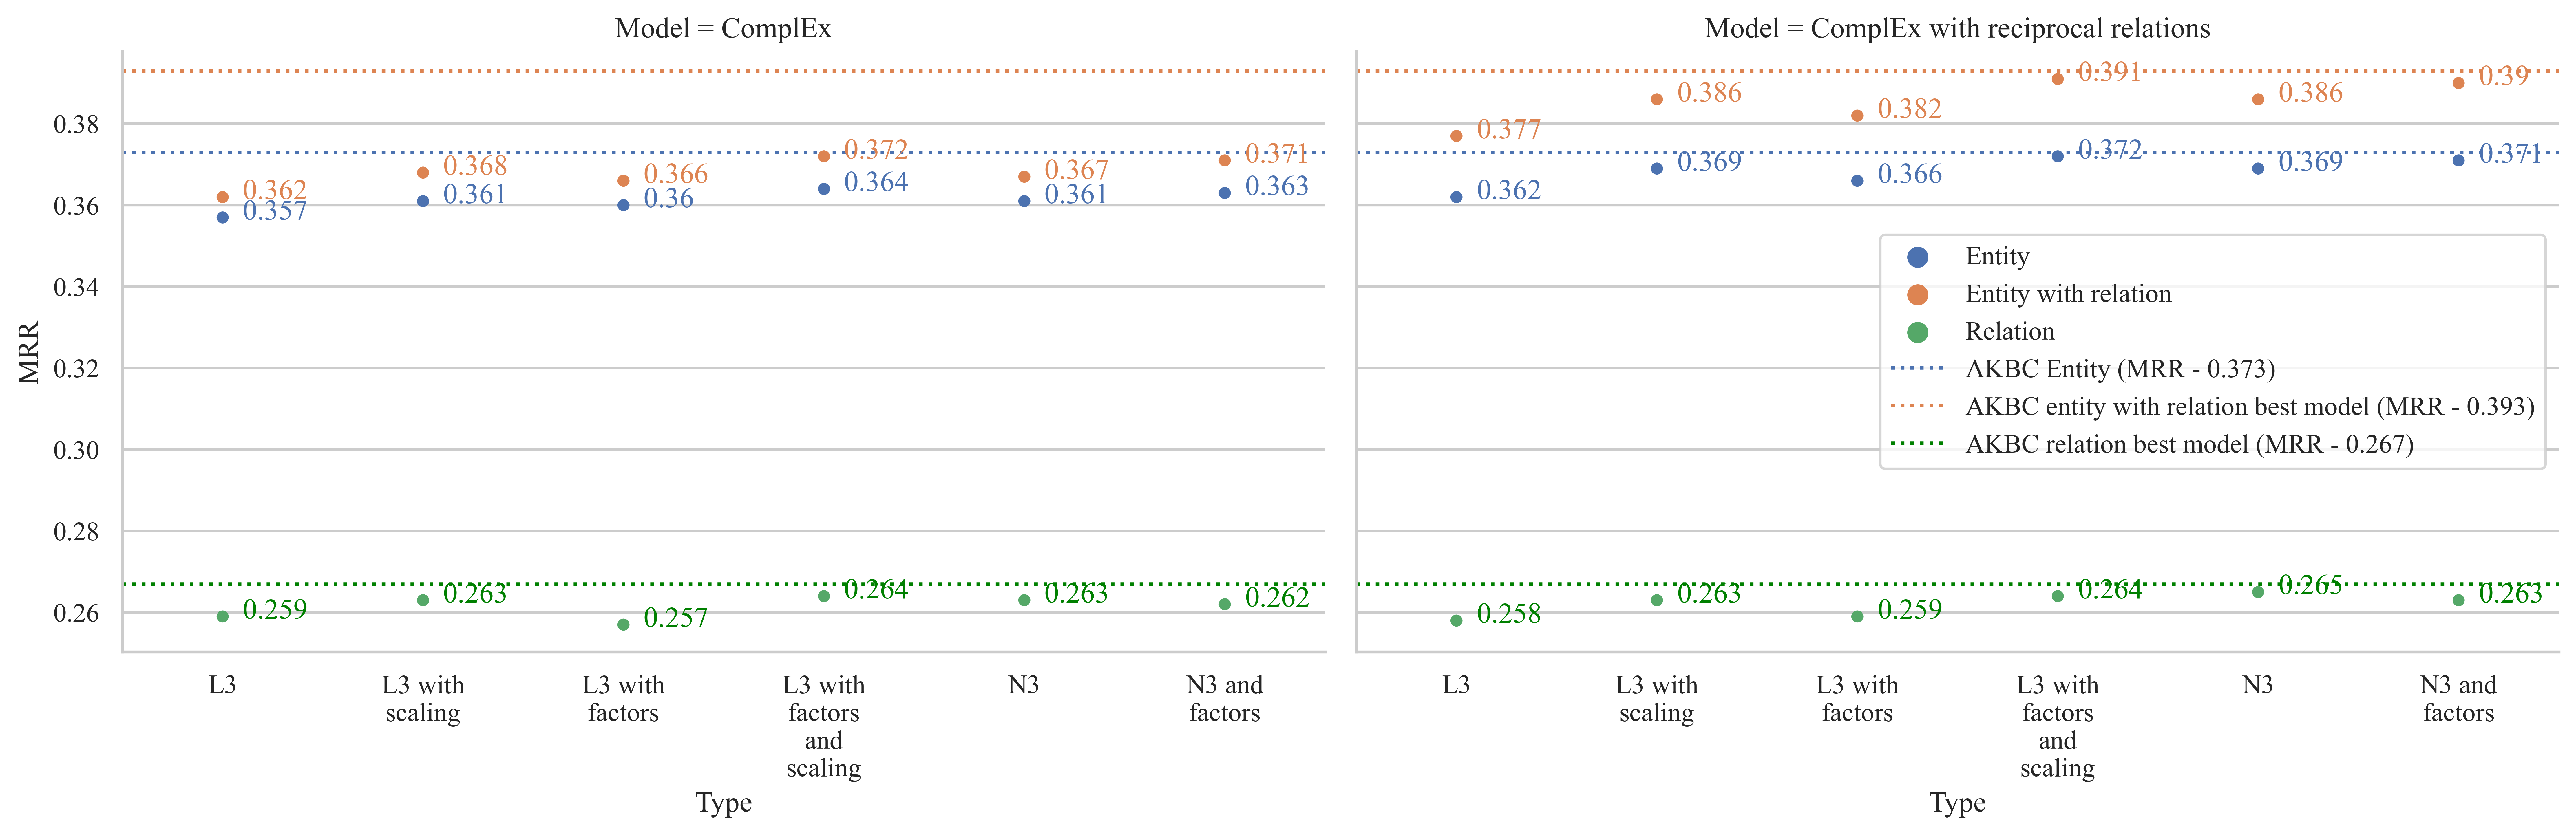
\includegraphics[width=\linewidth]{Images/Ablation_FB237.png}
	\caption[Performance of model when applying changes on FB15K-237]{Performance of model when applying changes on FB15K-237. \textit{Type:} indicates the changes has been applied}
	\label{fig:Ablation FB237}
	\end{center}
\end{figure}


The results for ablation study are shown in Figures \ref{fig:Ablation FB237} and \ref{fig:Ablation WNRR} respectively. The orange represents the performance of models trained on hybrid training objective, while the blue represent for models trained on standard training objective. The green is for models trained on relation training objective. The lines illustrate the performance from \citet{chen2021relation}'s models. The "type"-axis represents the changes that were applied to the models. "Normal weight" means that models were trained with the same-value weights as reported in the papers. "Scaled weight" means the regularization weights were scaled based on the difference in the implementation between two codebases. "Complex emb. vector" means that embedding vectors were considered as complex vector when performing penalty calculation.


On FB15K-237, the Figure \ref{fig:Ablation FB237} demonstrates, by using reciprocal relation technique, the performance of model on entity prediction (entity MRR) was boosted, i.e., MRR increases 1\% or 2\% (from 36.2\% to 37.7\%). Furthermore, with unexplored regularization weights, the models could achieve must more better results (37.7\% to 38.6\% MRR). 

However, the main difference between LibKGE and \citet{chen2021relation}'s codebase, i.e., considering embedding vector as complex vectors could slightly improve MRR by around 0.5\%. Clearly seen that, the main improvement comes from unexplored regularization weights and it does not matter how we treat the embedding vector as complex vector or not. 

\begin{figure}[!htbp]
	\begin{center}
	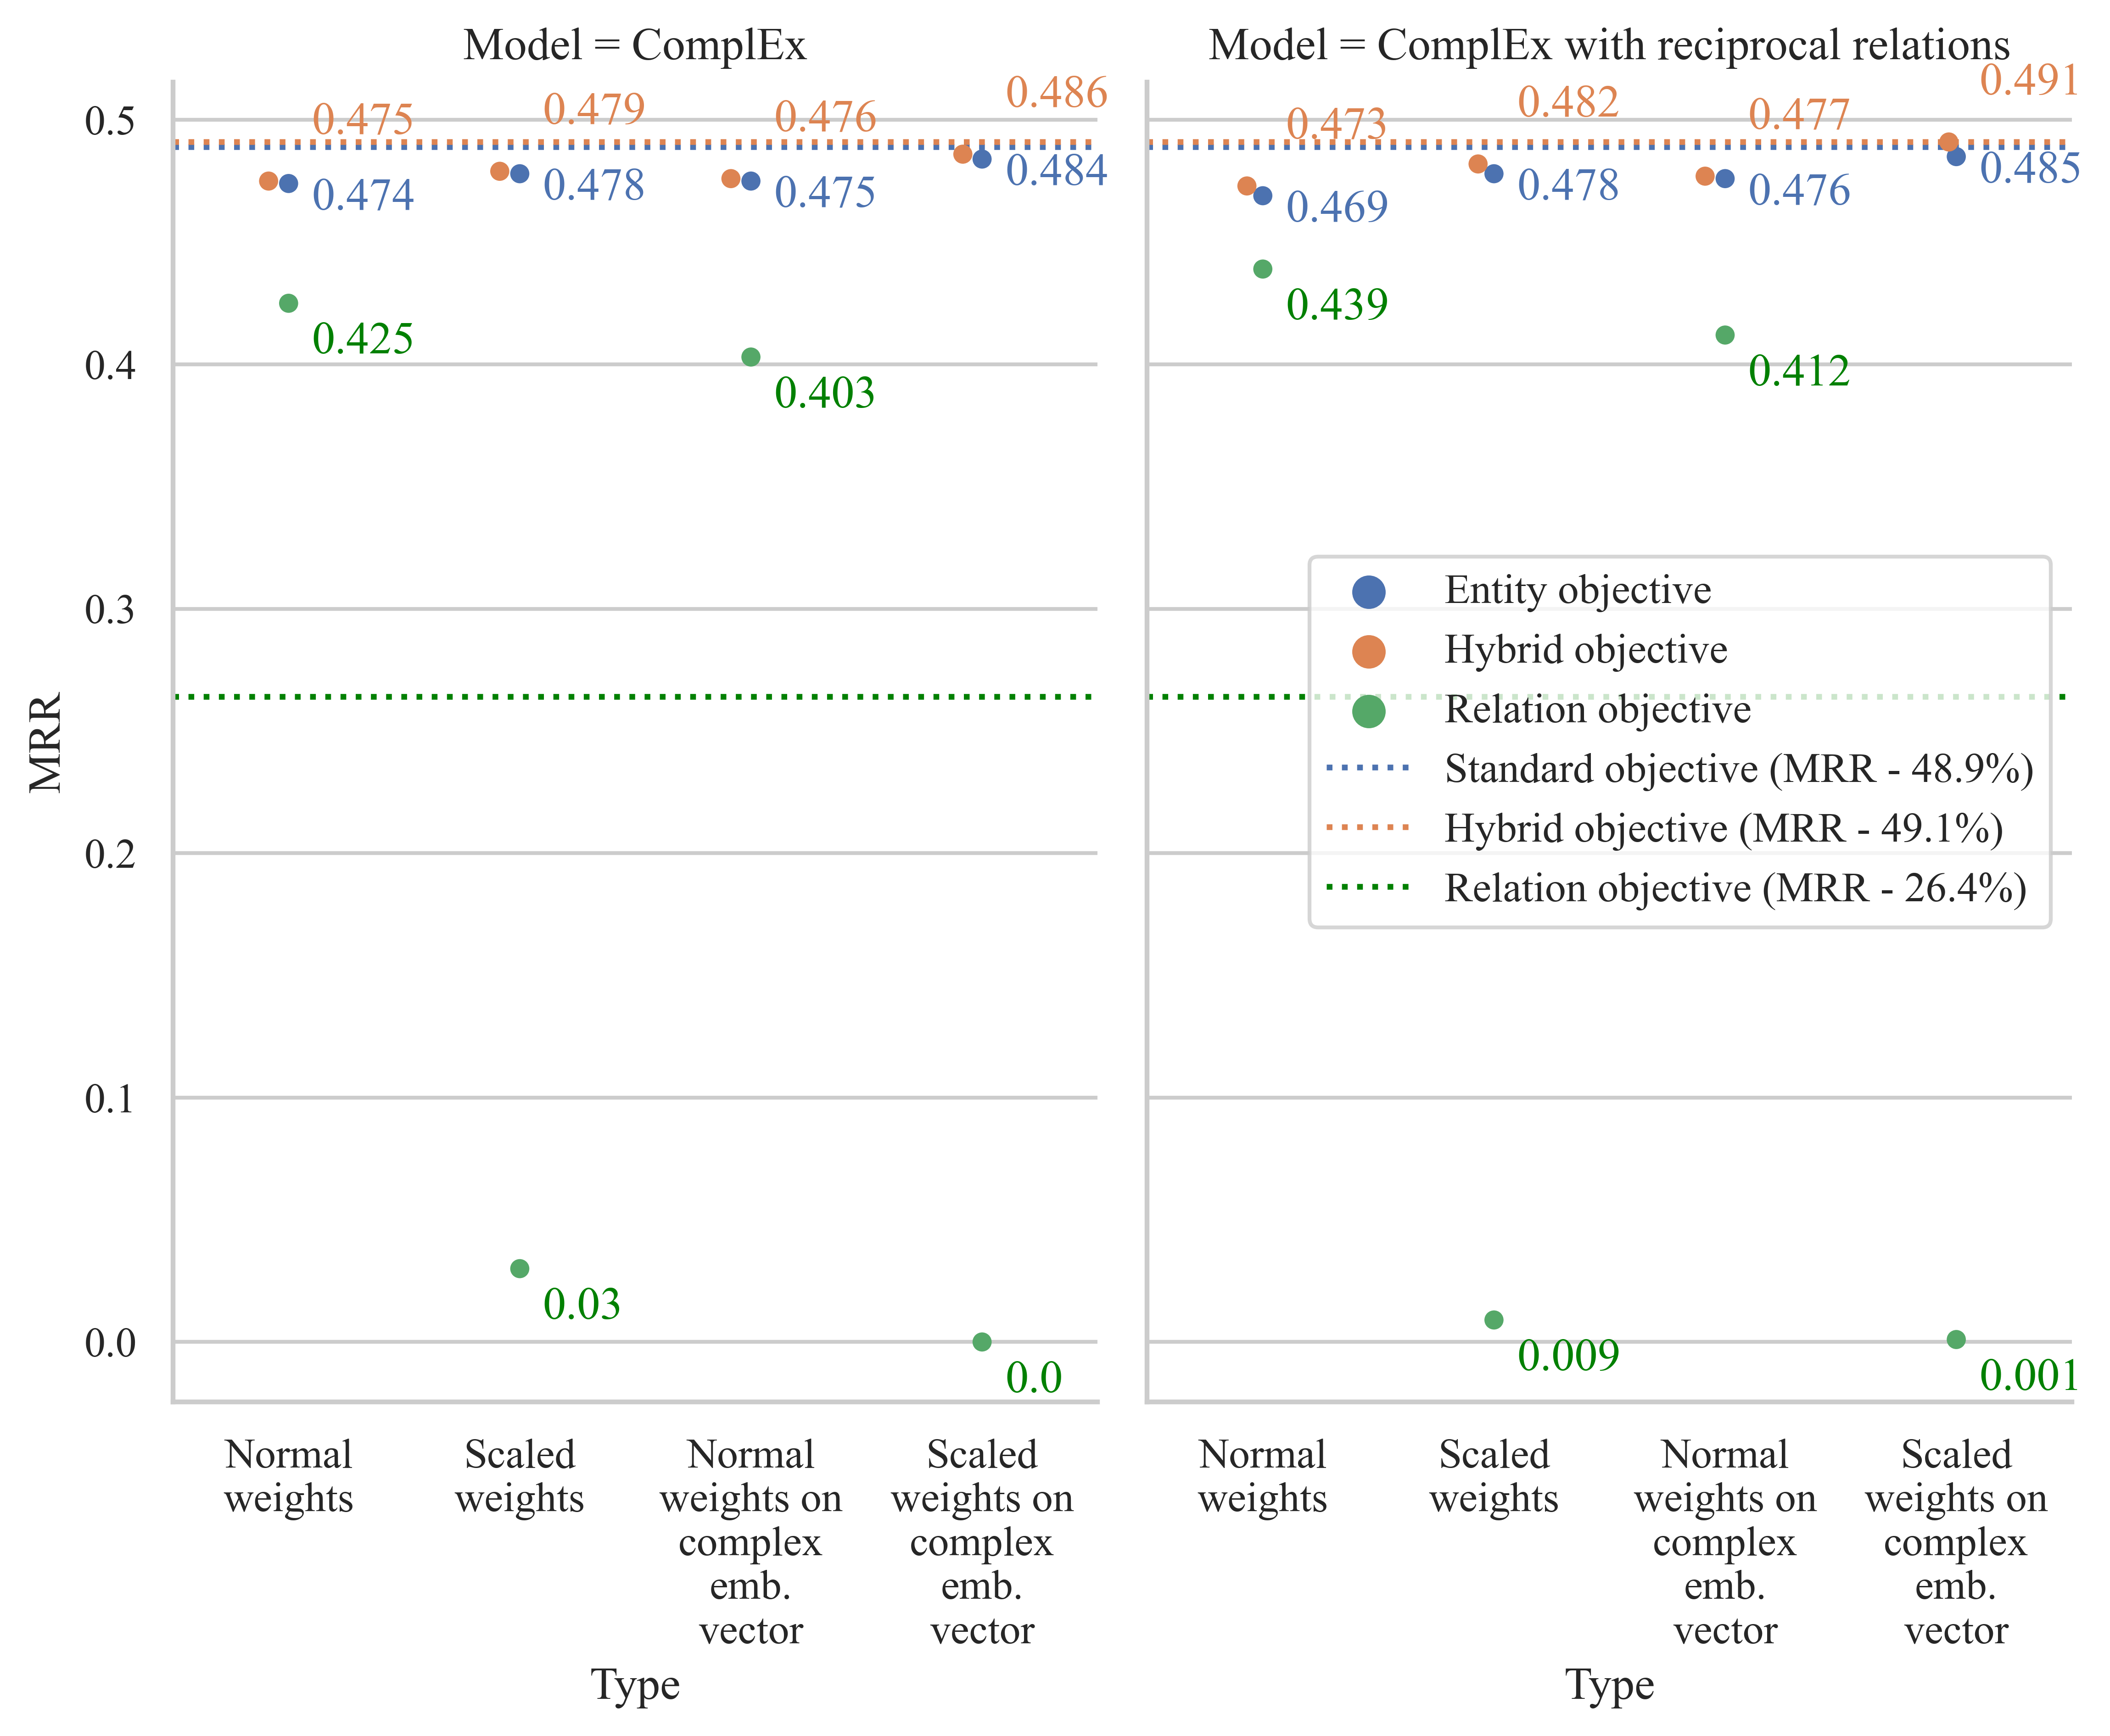
\includegraphics[width=\linewidth]{Images/Ablation_WNRR.png}
	\caption[Performance of model when applying changes on WN18RR]{Performance of model when applying changes on WN18RR. \textit{Type:} indicates the changes has been applied}
	\label{fig:Ablation WNRR}
	\end{center}
\end{figure}

On WN18RR, Figures \ref{fig:Ablation WNRR} states that the improvement is not really clear. However, we can see the same pattern as we observed on FB15K-237, with the unexplored regularization weights, the model trained on standard and hybrid objectives could achieve much more better results in entity MRR, that is 48.6\% and 48.4\% vs 47.6\% and 47.5\% without reciprocal technique and 49.1\% and 48.5\% vs 47.7\% and 47.6\% with reciprocal relations.
\newline

\noindent\textbf{Complex embedding vector in unrestricted HPC space.} The HPC space from \citet{chen2021relation} is a restricted space with numerous predefined hyperparameters such as regularizer, embedding initialization method or training optimizer. Therefore, we conducted an experiment on an unrestricted HPC space to observe the effect of considering embedding vectors as complex vectors in penalty calculation. The unrestricted HPC space we chose is from \citet{Ruffinelli2020You}. 

\begin{table}[!htbp]
\centering
\resizebox{\textwidth}{!}{%
\begin{tabular}{@{}lcccllll@{}}
\toprule
\textbf{Dataset} & \multicolumn{1}{l}{\textbf{Relation}} & \multicolumn{1}{l}{\textbf{Entity}} & \textbf{Complex vector} & \textbf{MRR} & \textbf{Hits@1} & \textbf{Hits@3} & \textbf{Hits@10} \\ \midrule
FB15K-237 & No & Yes & Yes & 34.9 & 26.2 & 38.0 & 52.3 \\
 & No & Yes & No & 35.0 & 26.1 & 38.3 & 52.8 \\ \cmidrule(l){2-8} 
 & Yes & Yes & Yes & 35.0 & 26.6 & 38.0 & 51.5 \\
 & Yes & Yes & No & 35.1 & 26.4 & 38.2 & 52.9 \\ \midrule
WN18RR & No & Yes & Yes & 47.6 & 44.5 & 48.6 & 54.0 \\
 & No & Yes & No & 47.6 & 44.4 & 48.9 & 53.8 \\ \cmidrule(l){2-8} 
 & Yes & Yes & Yes & 46.2 & 43.5 & 47.3 & 51.2 \\
 & Yes & Yes & No & 46.5 & 43.9 & 47.5 & 51.5 \\ \bottomrule
\end{tabular}%
}
\caption[Effect of considering embedding vectors as complex vectors]{The performance of models in FB15K-237 and WN18RR with and without considering embedding vectors as complex vectors. The \textit{Complex vector} indicates that considering the embedding vector as complex vector in penalty calculation. \textit{Yes} value means model considered embedding vectors as complex vectors while \textit{No} value means model does not consider embedding vectors as complex vectors. }
\label{tab:ICLR factor matter}
\end{table}

Table \ref{tab:ICLR factor matter} reports the models' performance with and without considering embedding vectors as complex vectors on unrestricted HPC space. From the table we can note that there is no difference between with or without the consideration. Therefore the main improvement come from unexplored values in the HPC space. 

\section[Finding ability of LibKGE]{Ability of finding \cite{chen2021relation}'s best models}

In this chapter, we reported the differences between two codebase and we have found exactly the configuration to reproduce the best models from \cite{chen2021relation} using LibKGE. However, the main question now is that we can find those models using Random Search approach in LibKGE or those models that are too good to be found. 

\begin{table}[!htbp]
\centering
\resizebox{0.9\textwidth}{!}{%
\begin{tabular}{@{}llll@{}}
\toprule
Trial & Hyperparameter & Values & entity MRR \\ \midrule
1 & Embedding initialization & Normal & 39.1 \\
 & Std. deviation (Normal) & 0.001 &  \\
 & Lp regularization & L3 &  \\
 & Entity emb. weight & {[}0.0005, 1.0{]}, log scale &  \\
 & Relation emb. weight & {[}0.0005, 1.0{]}, log scale &  \\ \midrule
2 & Embedding initialization & Normal & 39.0 \\
 & Std. deviation (Normal) & 0.001 &  \\
 & Lp regularization & \{L1, L2, L3, None\} &  \\
 & Entity emb. weight & {[}0.0005, 1.0{]}, log scale &  \\
 & Relation emb. weight & {[}0.0005, 1.0{]}, log scale &  \\ \midrule
2 & Embedding initialization & Normal & 38.9 \\
 & Std. deviation (Normal) & 0.001 &  \\
 & Lp regularization & \{L1, L2, L3, None\} &  \\
 & Entity emb. weight & {[}0.0005, 1.0{]}, log scale &  \\
 & Relation emb. weight & {[}0.0005, 1.0{]}, log scale &  \\ \bottomrule
\end{tabular}%
}
\caption[Model performance when relaxing the restricted HPC space]{Model performance when relaxing the restricted HPC space. The \textit{Trial} indicates the id of trial, \textit{Hyperparameters} are the hyperparameters we attempted to relax with their corresponding values in the \textit{Value} column. Entity MRR indicates the MRR that the best model can achieve.}
\label{tab:finding ability}
\end{table}

Due to the huge difference between restricted HPC space from \cite{chen2021relation} and unrestricted HPC space from \cite{Ruffinelli2020You}, we relaxed the hyperparameter bit by bit. Within this scope of the study, we only focus on reproducing the model trained on the hybrid training objective, the best-performance model was selected on entity MRR. The model was trained on FB15K-237. Table \ref{tab:finding ability} shows the performance of the best models we found after 3 times relaxing the restricted HPC space (on entity MRR). 

As illustrated in the table, so far we still can find the best model from \cite{chen2021relation}. However, the range for regularization weight is still small $[0.0005, 1.0]$ compared to unrestricted HPC space i.e., close interval $[1.0^{-20}, 1.0^{-01}]$. Therefore, the future study should enlarge the close interval for regularization weight to test the finding ability of LibKGE.



\chapter{Comparative study}
\label{chap:comparative_study}

In this chapter, we reported on the design and results of our comparative study. We mainly compared the performance of the ComplEx model in different model selection and training objectives, but, in a similar setting. This chapter aims to answer two questions: (1) Does hybrid training improve the performance of a model in relation prediction? (2) What is the effect of using overall MRR instead of entity MRR in model selection.

\section{Experimental setup}

\noindent\textbf{Dataset.} Despite the popularity of the FB15K dataset, we used the FB15K-237 and WN18RR in our study because of three reasons: (i) they are "hard" datasets since they were explicitly designed to evaluate multi-relational link prediction, (ii) they are diverse in that models often yield different performance, (iii) they are of reasonable size for a large study \citep{Ruffinelli2020You}.
\newline


\noindent\textbf{Models.} Within the scope of this thesis, we mainly focused on the ComplEx model due to excessive training costs \citep{trouillon2016complex}. Focusing on the ComplEx model, we can directly compare our results with \citet{chen2021relation} and \citet{Ruffinelli2020You}. Furthermore, this model is also one of the most well-known KGE models, besides RESCAL \citep{nickel2011three}, TransE \citep{bordes2013translating}, and DisMult \citep{yang2014embedding}. 
% We also tried to run experiments on RotatE \citep{sun2019rotate}, since \citet{sun2019rotate} also considered the embedding vector as a complex vector, the results were reported in Appendix \ref{sec:RotatE performance}. 
\newline

\noindent\textbf{Evaluation metric.} We reported filtered MRR and filtered Hits@\{1, 3, 10\} on entity prediction and relation prediction. We used the validation dataset for analysis.
% , and the final results will be reported using test data (Table \ref{tab:Final results}).
\newline

\noindent\textbf{Loss function.} In this thesis, we used the CE loss function so as to be able to compare with \citet{chen2021relation}'s results and since \citet{Ruffinelli2020You} have shown that the use of CE yields to better configuration than other loss functions. 
\newline

\noindent\textbf{Relation weight.} In their experimental setup, \citet{chen2021relation} searched the weight of relation prediction over set \{0.005, 0.001, 0.05, 0.1, 0.5, 1\} for WN18RR, and for FB15k-237, they searched over set \{0.125, 0.25, 0.5, 1, 2, 4\}. To have only one comprehensive HPC space for both datasets, we combined both sets of weights and searched relation prediction over a closed interval $[0.005, 4.0]$, and we sampled the weights uniformly instead of using a log scale. 
\newline

\noindent\textbf{Hyperparameters configuration (HPC) space.} Our HPC space bears a close resemblance to the HPC space from \citet{Ruffinelli2020You}. The reason we chose their HPC space is that this hyperparameter space is not excluded from a prior hyperparameter and contains salient points. However, in our searching space, instead of using all three primary training objectives (NegSamp, 1vsAll, and KvsAll), we only focused on 1vsAll, so that we could directly study the effect of hybrid training proposed by \citet{chen2021relation}. Furthermore, embedding vectors were considered a real embedding vectors instead of complex vectors when performing penalty calculations. The details of the HPC space can be found in Table \ref{tab:experimental settings} in Appendix \ref{cha:details of experimental setting}.

We aware that \citet{chen2021relation}'s HPC space could yield better models than \citet{Ruffinelli2020You}'s HPC space in terms of entity ranking. However, due to a lack of resources and time, we had conducted the comparative study simultaneously with reproducibility, therefore the preliminary results from \cite{chen2021relation}'s HPC were discussed in Section \ref{sec: Hybrid training in AKBC HPC space}. Furthermore, we note that the searching space from \cite{chen2021relation} is restricted which could lead to bias, thus, the main focus of this comparative study is the HPC from \cite{Ruffinelli2020You}.
\newline


\noindent\textbf{Training.} All models were trained for a maximum of 400 epochs. Models were validated every five epochs on validation and we performed early stopping with a patience of 50 epochs which is similar to the setup of \citet{Ruffinelli2020You}.
\newline

\noindent\textbf{Metrics.} 
In this thesis, filtered MRR and filtered Hits@\{1, 3, 10\} are metrics used to evaluate the models in relation prediction and entity prediction, so we can be able to compare results with \citet{chen2021relation} and \citet{Ruffinelli2020You}. MR is not adopted, since it is sensitive to outliers \citep{nickel2016holographic}.
\newline

\noindent\textbf{Ranking in relation prediction task.} When applying the reciprocal technique, the number of relations is doubled and the score functions of $(i, k, j)$ and $(j, k, i)$ differs. Therefore given a true triple $(i, k, j)$, we note that two potential answers are depending on the order of subject and object in relation prediction tasks. However, to preserve the validation dataset, we only validated the $(i, ?, j)$ query and ignored the validation for the inverse query $(j, ?, i)$. Furthermore, all relations including the reciprocal relations, are considered during the evaluation protocol. 
\newline

\noindent\textbf{Model selection.} We studied the effect of model selection on three different MRRs: entity MRR, relation MRR and overall MRR (micro-average of entity and relation MRRs). All of them are filtered MRRs. 
\newline




\section[Training objectives]{Training objectives: entity, hybrid, and relation training objectives}
\label{sec:Training objectives}

The effect of three training objectives: entity, hybrid, and relation training objectives to relation prediction performance (i.e., filtered relation MRR) is the main discussion in this section. We selected the best-performance models based on filtered entity MRR. Table \ref{tab:ICLR RP on ER} shows the performance of the best models on relation prediction as well as entity prediction. The performance of model are reported using filtered MRR and filtered Hits@\{1, 3, 10\} 


\begin{table}[!htbp]
\centering
\resizebox{\textwidth}{!}{%
\begin{tabular}{@{}llllllllllll@{}}
\toprule
 &  &  & \multicolumn{4}{c}{\textbf{Entity prediction}} &  & \multicolumn{4}{c}{\textbf{Relation prediction}} \\ \cmidrule(lr){4-7} \cmidrule(l){9-12} 
\textbf{Dataset} & \textbf{Entity} & \textbf{Relation} & \textbf{MRR} & \textbf{Hits@1} & \textbf{Hits@3} & \textbf{Hits@10} &  & \textbf{MRR} & \textbf{Hits@1} & \textbf{Hits@3} & \textbf{Hits@10} \\ \midrule
FB15K-237 & Yes & No & 35.2 & 26.4 & 38.5 & 52.7 &  & 21.8 & 09.8 & 17.3 & 58.1 \\
 & Yes & Yes & 35.0 & 26.0 & 38.4 & 52.9 &  & 95.4 & 93.6 & 96.9 & 98.3 \\
 & No & Yes & 23.7 & 16.7 & 25.6 & 37.9 &  & 97.2 & 95.6 & 98.9 & 99.6 \\ \midrule
WN18RR & Yes & No & 46.9 & 43.8 & 48.0 & 52.7 &  & 76.0 & 66.1 & 80.5 & 99.9 \\
 & Yes & Yes & 46.6 & 43.3 & 48.4 & 52.6 &  & 67.2 & 54.5 & 75.4 & 85.9 \\
 & No & Yes & 43.6 & 41.2 & 44.5 & 48.0 &  & 63.1 & 49.5 & 71.5 & 82.3 \\ \bottomrule
\end{tabular}%
}
\caption[Model performance in three objectives (selected on entity MRR)]{Model performance in standard, hybrid and relation training objectives on FB15K-237 and WN18RR. The best models were selected on entity MRR. }
\label{tab:ICLR RP on ER}
\end{table}

Interestingly, as evidenced by Table \ref{tab:ICLR RP on ER}, in FB15K-237 dataset, by including negative examples which are obtained by perturbing the relation positions into 1vsAll (i.e., hybrid training objective), the performance of the model in terms of relation prediction was significantly improved. Model trained on hybrid objective achieved relation MRR of 95.4\% which is 4 times higher than model trained on standard objective i.e., relation MRR of 21.8\%. 

However, the effect of hybrid training objective was not observed in WN18RR, the performance of the model trained a hybrid training objective was relation MRR of 67.2\% which is 10\% lower than the relation MRR from model trained with a standard objective i.e., relation MRR of 76.0\%. Furthermore, we observed that training model by hybrid objective lowered the entity MRR from 46.9\% to 46.6\% - 3\% lower.

Table \ref{tab:ICLR RP on ER} additionally shows the models' performances when models were trained using negative relation examples only (relation training objective). By applying relation training objective, the ComplEx model can achieved the relation MRR of 97.2\% which is 2\% higher than the performance of model trained on hybrid training on FB15K-237. However, the performance on entity ranking dropped significantly to 23.7\% on entity MRR from 35.0\%. 

Furthermore, in WN18RR, there was an decrease in relation MRR performance when model trained on relation objective (i.e., from 67.2\% to 63.1\%), the same drop was also observed in entity MRR (from 46.6\% to 43.6\%). This trends were also observed in Hits@\{1, 3, 10\}.


One potential explanation for non-improvement when including negative relation examples in WN18RR would be that the dataset contains comparatively a small number of relation $|\mathcal{R}| = 11$ while the number of relation in FB15K-237 $|\mathcal{R}| = 237$. This observation was also reported by \cite{chen2021relation}. They found that hybrid training brings benefits to datasets with a larger number of predicates \citep{chen2021relation}.
\newline
 
 
\noindent\textbf{Relation prediction performance of \cite{chen2021relation}'s models.} The table \ref{tab:AKBC relation prediction} shows the performance of \citet{chen2021relation}'s best models on relation prediction and entity prediction. The results were produced using LibKGE. The table, one again, nicely illustrates the effect of hybrid training objective in relation prediction. 


\begin{table}[!htbp]
\centering
\resizebox{\textwidth}{!}{%
\begin{tabular}{@{}lllccccccccc@{}}
\toprule
          &                   &                     & \multicolumn{4}{c}{\textbf{Entity prediction}}                                        &  & \multicolumn{4}{c}{\textbf{Relation prediction}}                                      \\ \cmidrule(lr){4-7} \cmidrule(l){9-12} 
\textbf{Dataset}   & \textbf{Entity} & \textbf{Relation} & \textbf{MRR}            & \textbf{Hits@1}         & \textbf{Hits@3}         & \textbf{Hits@10}        &  & \textbf{MRR}            & \textbf{Hits@1}         & \textbf{Hits@3}         & \textbf{Hits@10}        \\ \midrule
FB15K-237 & Yes               & No                  & 37.2          & 27.8          & 40.9          & 56.3          &  & 90.2          & 85.0          & 94.7          & 97.6          \\
          & Yes               & Yes                 & 39.1          & 30.0          & 42.7          & 57.2          &  & 95.4          & 92.1          & 98.8          & 99.6          \\
          & No                & Yes                 & 26.2          & 18.7          & 28.7          & 40.7          &  & 95.0          & 91.3          & 98.4          & 99.5          \\ \midrule
WN18RR    & Yes               & No                  & 48.6          & 44.4          & 49.8          & 57.1          &  & 76.8          & 70.3          & 79.5          & 89.0          \\
          & Yes               & Yes                 & 48.6          & 44.6          & 49.7          & 57.3          &  & 62.9          & 42.7          & 79.0          & 88.6          \\
          & No                & Yes                 & 14.1          & 08.3          & 18.2          & 24.3          &  & 24.0          & 00.0          & 38.4          & 49.5          \\ \bottomrule
\end{tabular}%
}
% This was took from with_reciprocal_factors_scaling_er (with relation) - valid.txt files not the original files
\caption[The Chen et al.'s best models' performance on entity and relation prediction.]{The \citet{chen2021relation}'s best model performance on entity prediction and relation prediction. The results were produced by using LibKGE.}
\label{tab:AKBC relation prediction}
\end{table}

There is not only the improvement in entity MRR, the table \ref{tab:AKBC relation prediction} also shows the improvement in relation MRR when model was trained on hybrid training objective. Compared with standard training objective, hybrid model achieved relation MRR of 95.2\% which is 5\% higher than standard model (relation MRR of 90.2\%). 

Although, the hybrid training objective brings benefits to in FB15K-237, however, we also observed a 14\% dropout in WN18RR when we trained model with hybrid training objective (from 76.8\% to 62.9\%). This observation strengthen the point of view that the hybrid training objective can bring improvement in relation MRR to those datasets which have a significant number of predicates.  

Another interesting observation from the \cite{chen2021relation}'s models is that those models trained only on relation training objective could not achieve better results than model trained on hybrid training objective. This observation is contradicted to what we observed in unrestricted HPC space (Table \ref{tab:ICLR RP on ER})

Furthermore, when comparing the performance of hybrid training models found in unrestricted HPC space with \cite{chen2021relation}'s best models (Table \ref{tab:ICLR RP on ER} and \ref{tab:AKBC relation prediction}), we observed that there is no difference between those two model in relation prediction performance. This indicates that \cite{chen2021relation}'s best models is more suitable for entity prediction than relation prediction.
\newline



% \textbf{Should we conduct an ablation study for this?}

\noindent\textbf{Positive impact of hybrid training.} The evidence from observing the performance of models trained on hybrid training objective points towards the idea that this training objective could bring a nice benefit not only for entity prediction (on \citet{chen2021relation}'s HPC space), but also for relation prediction (on both HPC spaces), although we chosen the best models in favor for entity prediction. Therefore, in the next section, we attempt to observe the performance of models when we select the best models in favor for both entity prediction and relation prediction (overall MRR). 



\section[Model selection]{Model selection: entity MRR, overall MRR, relation MRR}

In the previous section, we observed that using a hybrid training objective leads to improvement of the model's performance in relation prediction. However, the best models were selected based on the entity MRR which is mainly focusing on the performance of mode in entity ranking. Therefore, in this section, the models will be selected on overall MRR which is the micro-average between subject MRR, object MRR and relation MRR (details in Equation \ref{eq:overall MRR}). Table \ref{tab:ICLR RP on ER vs Hybrid} shows the comparison between two model selection approaches, the performance was represented by filter MRRs (for other metrics, see Table \ref{tab:Full ICLR results}). 


\begin{table}[!htbp]
\centering
\resizebox{\textwidth}{!}{%
\begin{tabular}{@{}llllllll@{}}
\toprule
 &  &  & \multicolumn{2}{c}{\textbf{Selected on entity MRR}} & \textbf{} & \multicolumn{2}{c}{\textbf{Selected on overall MRR}} \\ \cmidrule(lr){4-5} \cmidrule(l){7-8} 
\textbf{Dataset} & \textbf{Entity} & \textbf{Relation} & \textbf{entity MRR} & \textbf{relation MRR} &  & \textbf{entity MRR} & \textbf{relation MRR} \\ \midrule
FB15K-237 & Yes & No & 35.2 & 21.8 &  & 33.5 & 89.4 \\
 & Yes & Yes & 35.0 & 95.4 &  & 34.6 & 96.8 \\
 & No & Yes & 23.7 & 97.2 &  & 24.0 & 97.4 \\ \midrule
WN18RR & Yes & No & 46.9 & 76.0 &  & 45.2 & 88.8 \\
 & Yes & Yes & 46.6 & 67.2 &  & 42.6 & 80.8 \\
 & No & Yes & 43.6 & 63.1 &  & 42.7 & 63.5 \\ \bottomrule
\end{tabular}%
}
\caption[Model performance in three training objectives (selected on entity and overall MRRs)]{Model performance in three training objectives. \textit{Selected on entity MRR:} The best models were selected based on models' performance in entity MRR metric. \textit{Selected on overall MRR:} The best models were selected based on models' performance in overall MRR metric.}
\label{tab:ICLR RP on ER vs Hybrid}
\end{table}


As was mentioned in the previous section (section \ref{sec:Training objectives}), the model trained on standard training objective can only achieve 21.8\% of relation MRR. However, as can be seen in Table \ref{tab:ICLR RP on ER vs Hybrid}, without training from scratch, we can obtain a better model in relation prediction (89.4\% in relation MRR) by selecting the best models on overall MRR instead of on entity MRR. Interestingly, this positive effect also can be observed on WN18RR also. The best model can achieve up to relation MRR of 88.8\% instead of 76.0\%. However, there is a trade-off when selecting best-performance models on overall MRR, the model's performance in entity prediction dropped notably by around 2\% on both dataset. 

To overcome that trade-off, as shown in \ref{tab:ICLR RP on ER vs Hybrid}, if we re-train models on hybrid training objective, the drop in entity ranking become smaller, instead of 2\%, now it only about 0.4\%. Furthermore, the model can now even achieve higher relation MRR (96.8\% instead of 95.4\% on FB15K-237). 

Unfortunately, that trend was not observed on WN18RR. We still observe the non-improvement even if we select a model based on overall MRR. The performance reduce from 88.8\% to 80.8\% along with the reduce in entity ranking performance also from 45.2\% ti 42.6\%

Based on those observations, we can conclude that the model selection positively affect the model's performance if the model is trained on a hybrid training objective on unrestricted HPC space. 
\newline

\noindent\textbf{Relation MRR}: It is easy to see from Table \ref{tab:ICLR RP on ER vs Hybrid vs relation}, selecting a model on relation MRR brings better performance on relation prediction, but, at the same time, the models underperformed on entity prediction.  

% Please add the following required packages to your document preamble:
% \usepackage{booktabs}
% \usepackage{graphicx}
\begin{table}[!htbp]
\centering
\resizebox{\textwidth}{!}{%
\begin{tabular}{@{}lllllllllll@{}}
\toprule
 &  &  & \multicolumn{2}{c}{\textbf{Selected on entity MRR}} & \textbf{} & \multicolumn{2}{c}{\textbf{Selected on overall MRR}} & \textbf{} & \multicolumn{2}{c}{\textbf{Selected on relation MRR}} \\ \cmidrule(lr){4-8} \cmidrule(l){10-11} 
\textbf{Dataset} & \textbf{Entity} & \textbf{Relation} & \textbf{entity MRR} & \textbf{relation MRR} &  & \textbf{entity MRR} & \textbf{relation MRR} &  & \textbf{entity MRR} & \textbf{relation MRR} \\ \midrule
FB15K-237 & Yes & No & 35.2 & 21.8 &  & 33.5 & 89.4 &  & 30.9 & 92.9 \\
 & Yes & Yes & 35.0 & 95.4 &  & 34.6 & 96.8 &  & 32.0 & 97.3 \\
 & No & Yes & 23.7 & 97.2 &  & 24.0 & 97.4 &  & 17.9 & 97.8 \\ \midrule
WN18RR & Yes & No & 46.9 & 76.0 &  & 45.2 & 88.8 &  & 45.6 & 89.4 \\
 & Yes & Yes & 46.6 & 67.2 &  & 42.6 & 80.8 &  & 40.0 & 89.3 \\
 & No & Yes & 43.6 & 63.1 &  & 42.7 & 63.5 &  & 02.1 & 90.8 \\ \bottomrule
\end{tabular}%
}
\caption[Model performance in three training objectives (selected on entity, overall and relation MRRs)]{Model performance in three training objectives. \textit{Selected on entity MRR:} The best models were selected based on models' performance in entity MRR metric.
\textit{Selected on overall MRR:} The best models were selected based on models' performance in overall MRR metric. \textit{Selected on relation MRR:} The best models were selected based on models' performance in relation MRR metric.}
\label{tab:ICLR RP on ER vs Hybrid vs relation}
\end{table}


\section[Primary results of Chen et al. (2021)]{Primary results \cite{chen2021relation}'s HPC space}
\label{sec: Hybrid training in AKBC HPC space}
Due to the restricted time for a master thesis, we conducted the comparative study simultaneously with the reproducing phase (Chapter \ref{chap:reproducibility}). Therefore, the awareness about reciprocal techniques and the difference in L3 implementation were absent on the time this experiment conducted. Thus, we studied the \cite{chen2021relation}'s HPC space without applying the reciprocal technique. Furthermore, when calculate the regularization for embedding, we consider embedding vectors as real vector. i.e., the vectors in real vector space.   
\newline

\noindent\textbf{Semi-restricted HPC space.} We would like to call this HPC space is semi-restricted HPC space due to the following restrictions. To imitate the \cite{chen2021relation}'s HPC space, we use Adagrad as optimizer, learning rate without log scale, and normal distribution as embedding initialization methods with $\mu=0$ and $\sigma=0.001$. Additionally, penalty for the embedding of an object is weighted by the object's frequency in the training data i.e., the frequency weighting is true. For another hyperparameters, we keep them as same as values in \citet{Ruffinelli2020You}'s HPC space such as learning scheduler, the number of epochs and the early-stopping criteria (see Table \ref{tab:experimental settings} in Appendix \ref{cha:details of experimental setting} for details).  

For important hyperparameters, we merged the values from \citet{Ruffinelli2020You}'s HPC space and values from \cite{chen2021relation}'s HPC space together. Furthermore, the searching range for relation weight is enlarged from $[0.005, 4.0]$ to $[0.1, 8.0]$. Table \ref{tab:Searching space to find AKBC} shows the values for important hyperparameters. This is also the HPC space that we used to find \citet{chen2021relation}'s best models (in section \ref{sec:Similarly setting}) and we also unitized this HPC space to study impact of hybrid training on larger embedding size.


\begin{table}[!htbp]
\centering
\resizebox{\textwidth}{!}{%
\begin{tabular}{@{}lllllllllll@{}}
\toprule
 &  &  & \multicolumn{2}{c}{\textbf{Selected on entity MRR}} & \textbf{} & \multicolumn{2}{c}{\textbf{Selected on overall MRR}} & \textbf{} & \multicolumn{2}{c}{\textbf{Selected on relation MRR}} \\ \cmidrule(lr){4-8} \cmidrule(l){10-11} 
\textbf{Dataset} & \textbf{Entity} & \textbf{Relation} & \textbf{entity MRR} & \textbf{relation MRR} &  & \textbf{entity MRR} & \textbf{relation MRR} &  & \textbf{entity MRR} & \textbf{relation MRR} \\ \midrule
FB15K-237 & Yes & No & 36.6 & 94.7 &  & 36.5 & 94.9 &  & 35.5 & 95.0 \\
 & Yes & Yes & 37.3 & 97.9 &  & 37.1 & 98.0 &  & 36.5 & 98.0 \\
 & No & Yes & 25.8 & 96.2 &  & 25.8 & 96.4 &  & 17.3 & 97.8 \\ \midrule
WN18RR & Yes & No & 47.9 & 83.7 &  & 48.0 & 83.9 &  & 48.1 & 84.8 \\
 & Yes & Yes & 48.1 & 86.0 &  & 48.1 & 86.1 &  & 36.3 & 90.2 \\
 & No & Yes & 45.8 & 80.9 &  & 45.2 & 87.8 &  & 40.0 & 89.2 \\ \bottomrule
\end{tabular}%
}
\caption[Model performance in three training objectives on semi-restricted HPC space (selected on entity, overall and relation MRRs)]{Model performance in three training objectives on semi-restricted HPC space. \textit{Selected on entity MRR:} The best models were selected based on models' performance in entity MRR metric.
\textit{Selected on overall MRR:} The best models were selected based on models' performance in overall MRR metric. \textit{Selected on relation MRR:} The best models were selected based on models' performance in relation MRR metric. (for other metrics, see Table \ref{tab:Full AKBC results})}
\label{tab:Semi-retricted HPC results}
\end{table}


Table \ref{tab:Semi-retricted HPC results} illustrates the benefit of using hybrid training objective which are consistent with previous results illustrated in Table \ref{tab:Semi-retricted HPC results} and Table \ref{tab:ICLR RP on ER vs Hybrid vs relation}. Surprisingly, on this semi-restricted HPC space, the effect of model selection is not observed anymore. 

We can clearly observe that the performance of models on entity and relation prediction are consistent regardless of model selection. When we trained model on hybrid training objective on FB15K-237, model can achieve 37.3\% entity MRR and 97.9\% relation MRR which are higher than entity MRR and relation MRR standard model can achieve (36.6\% and 94.7\% resp.).  

Unsurprisingly, by comparing Table \ref{tab:Semi-retricted HPC results} and Table \ref{tab:ICLR RP on ER vs Hybrid vs relation}, the semi-restricted HPC space yield better models than unrestricted HPC space (i.e., the HPC space from \cite{Ruffinelli2020You}).



\section{Conclusion}
Our comparative study has led us to conclude that hybrid training objective could bring a positive effect to ComplEx model not only on predicting entity but also relation prediction. Furthermore, model selection could become handy for ComplEx mode to obtain better model on relation prediction without training from scratch.  

% The model should be trained on a hybrid training objective to achieve good performance on entity ranking and relation prediction. The performance of the model on test data was reported in Table \ref{tab:Final results}




\chapter{Theoretical Framework}
\label{cha:theory}

But I must explain to you how all this mistaken idea of denouncing pleasure and praising pain was born and I will give you a complete account of the system, and expound the actual teachings of the great explorer of the truth, the master-builder of human happiness. No one rejects, dislikes, or avoids pleasure itself, because it is pleasure, but because those who do not know how to pursue pleasure rationally encounter consequences that are extremely painful. Nor again is there anyone who loves or pursues or desires to obtain pain of itself, because it is pain, but because occasionally circumstances occur in which toil and pain can procure him some great pleasure. To take a trivial example, which of us ever undertakes laborious physical exercise, except to obtain some advantage from it? But who has any right to find fault with a man who chooses to enjoy a pleasure that has no annoying consequences, or one who avoids a pain that produces no resultant pleasure?

On the other hand, we denounce with righteous indignation and dislike men who are so beguiled and demoralized by the charms of pleasure of the moment, so blinded by desire, that they cannot foresee the pain and trouble that are bound to ensue; and equal blame belongs to those who fail in their duty through weakness of will, which is the same as saying through shrinking from toil and pain. These cases are perfectly simple and easy to distinguish. In a free hour, when our power of choice is untrammelled and when nothing prevents our being able to do what we like best, every pleasure is to be welcomed and every pain avoided. But in certain circumstances and owing to the claims of duty or the obligations of business is will frequently occur that pleasures have to be repudiated and annoyances accepted. The wise man therefore always holds in these matters to this principle of selection: he rejects pleasures to secure other greater pleasures, or else he endures pains to avoid worse pains. 


\section{Preliminaries}
\label{sec:prelim}

But I must explain to you how all this mistaken idea of denouncing pleasure and praising pain was born and I will give you a complete account of the system, and expound the actual teachings of the great explorer of the truth, the master-builder of human happiness. No one rejects, dislikes, or avoids pleasure itself, because it is pleasure, but because those who do not know how to pursue pleasure rationally encounter consequences that are extremely painful. Nor again is there anyone who loves or pursues or desires to obtain pain of itself, because it is pain, but because occasionally circumstances occur in which toil and pain can procure him some great pleasure. To take a trivial example, which of us ever undertakes laborious physical exercise, except to obtain some advantage from it? But who has any right to find fault with a man who chooses to enjoy a pleasure that has no annoying consequences, or one who avoids a pain that produces no resultant pleasure?

Notice that your theoretical framework should be less trivial than the following one. In most cases a definition requires some explanations. In particular, you should only introduce a definition if the subject under dicussion requires a precise definition.
\begin{definition}
\label{def:good}
An entity is good if it is not an evil entity.
\end{definition}
In a similar way an evil entity can be defined in the following way.
\begin{definition}
\label{def:evil}
An entity is evil if it is not a good entity.
\end{definition}
Proposition \ref{pro:good-evil} follows directly from Definition \ref{def:good} and \ref{def:evil}.
\begin{proposition}
\label{pro:good-evil}
There exists no such entity that is evil and good at the same time.
\end{proposition}



But I must explain to you how all this mistaken idea of denouncing pleasure and praising pain was born and I will give you a complete account of the system, and expound the actual teachings of the great explorer of the truth, the master-builder of human happiness. No one rejects, dislikes, or avoids pleasure itself, because it is pleasure, but because those who do not know how to pursue pleasure rationally encounter consequences that are extremely painful. Nor again is there anyone who loves or pursues or desires to obtain pain of itself, because it is pain, but because occasionally circumstances occur in which toil and pain can procure him some great pleasure. To take a trivial example, which of us ever undertakes laborious physical exercise, except to obtain some advantage from it? But who has any right to find fault with a man who chooses to enjoy a pleasure that has no annoying consequences, or one who avoids a pain that produces no resultant pleasure?



On the other hand, we denounce with righteous indignation and dislike men who are so beguiled and demoralized by the charms of pleasure of the moment, so blinded by desire, that they cannot foresee the pain and trouble that are bound to ensue; and equal blame belongs to those who fail in their duty through weakness of will, which is the same as saying through shrinking from toil and pain. These cases are perfectly simple and easy to distinguish. In a free hour, when our power of choice is untrammelled and when nothing prevents our being able to do what we like best, every pleasure is to be welcomed and every pain avoided. But in certain circumstances and owing to the claims of duty or the obligations of business is will frequently occur that pleasures have to be repudiated and annoyances accepted. The wise man therefore always holds in these matters to this principle of selection: he rejects pleasures to secure other greater pleasures, or else he endures pains to avoid worse pains. 

\section{The Good}
\label{sec:good}

But I must explain to you how all this mistaken idea of denouncing pleasure and praising pain was born and I will give you a complete account of the system, and expound the actual teachings of the great explorer of the truth, the master-builder of human happiness. No one rejects, dislikes, or avoids pleasure itself, because it is pleasure, but because those who do not know how to pursue pleasure rationally encounter consequences that are extremely painful. Nor again is there anyone who loves or pursues or desires to obtain pain of itself, because it is pain, but because occasionally circumstances occur in which toil and pain can procure him some great pleasure. To take a trivial example, which of us ever undertakes laborious physical exercise, except to obtain some advantage from it? But who has any right to find fault with a man who chooses to enjoy a pleasure that has no annoying consequences, or one who avoids a pain that produces no resultant pleasure?

\begin{figure}
	\begin{center}
	
\includegraphics[width=5cm]{good.png}
	\caption[Angel]{Child Angel and a white dove.}
	\label{fig:angel}
	\end{center}
\end{figure}

On the other hand, we denounce with righteous indignation and dislike men who are so beguiled and demoralized by the charms of pleasure of the moment, so blinded by desire, that they cannot foresee the pain and trouble that are bound to ensue; and equal blame belongs to those who fail in their duty through weakness of will, which is the same as saying through shrinking from toil and pain. These cases are perfectly simple and easy to distinguish. In a free hour, when our power of choice is untrammelled and when nothing prevents our being able to do what we like best, every pleasure is to be welcomed and every pain avoided. But in certain circumstances and owing to the claims of duty or the obligations of business is will frequently occur that pleasures have to be repudiated and annoyances accepted. The wise man therefore always holds in these matters to this principle of selection: he rejects pleasures to secure other greater pleasures, or else he endures pains to avoid worse pains. 

But I must explain to you how all this mistaken idea of denouncing pleasure and praising pain was born and I will give you a complete account of the system, and expound the actual teachings of the great explorer of the truth, the master-builder of human happiness. No one rejects, dislikes, or avoids pleasure itself, because it is pleasure, but because those who do not know how to pursue pleasure rationally encounter consequences that are extremely painful. Nor again is there anyone who loves or pursues or desires to obtain pain of itself, because it is pain, but because occasionally circumstances occur in which toil and pain can procure him some great pleasure. To take a trivial example, which of us ever undertakes laborious physical exercise, except to obtain some advantage from it? But who has any right to find fault with a man who chooses to enjoy a pleasure that has no annoying consequences, or one who avoids a pain that produces no resultant pleasure?

On the other hand, we denounce with righteous indignation and dislike men who are so beguiled and demoralized by the charms of pleasure of the moment, so blinded by desire, that they cannot foresee the pain and trouble that are bound to ensue; and equal blame belongs to those who fail in their duty through weakness of will, which is the same as saying through shrinking from toil and pain. These cases are perfectly simple and easy to distinguish. In a free hour, when our power of choice is untrammelled and when nothing prevents our being able to do what we like best, every pleasure is to be welcomed and every pain avoided. But in certain circumstances and owing to the claims of duty or the obligations of business is will frequently occur that pleasures have to be repudiated and annoyances accepted. The wise man therefore always holds in these matters to this principle of selection: he rejects pleasures to secure other greater pleasures, or else he endures pains to avoid worse pains. 

\section{The Evil}
\label{sec:evil}

But I must explain to you how all this mistaken idea of denouncing pleasure and praising pain was born and I will give you a complete account of the system, and expound the actual teachings of the great explorer of the truth, the master-builder of human happiness. No one rejects, dislikes, or avoids pleasure itself, because it is pleasure, but because those who do not know how to pursue pleasure rationally encounter consequences that are extremely painful. Nor again is there anyone who loves or pursues or desires to obtain pain of itself, because it is pain, but because occasionally circumstances occur in which toil and pain can procure him some great pleasure. To take a trivial example, which of us ever undertakes laborious physical exercise, except to obtain some advantage from it? But who has any right to find fault with a man who chooses to enjoy a pleasure that has no annoying consequences, or one who avoids a pain that produces no resultant pleasure?

On the other hand, we denounce with righteous indignation and dislike men who are so beguiled and demoralized by the charms of pleasure of the moment, so blinded by desire, that they cannot foresee the pain and trouble that are bound to ensue; and equal blame belongs to those who fail in their duty through weakness of will, which is the same as saying through shrinking from toil and pain. These cases are perfectly simple and easy to distinguish. In a free hour, when our power of choice is untrammelled and when nothing prevents our being able to do what we like best, every pleasure is to be welcomed and every pain avoided. But in certain circumstances and owing to the claims of duty or the obligations of business is will frequently occur that pleasures have to be repudiated and annoyances accepted. The wise man therefore always holds in these matters to this principle of selection: he rejects pleasures to secure other greater pleasures, or else he endures pains to avoid worse pains. 

\begin{figure}
	\begin{center}
	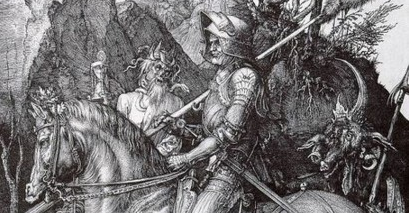
\includegraphics[width=\linewidth]{evil.png}
	\caption[Devil]{Knight and Devil.}
	\label{fig:devil}
	\end{center}
\end{figure}

But I must explain to you how all this mistaken idea of denouncing pleasure and praising pain was born and I will give you a complete account of the system, and expound the actual teachings of the great explorer of the truth, the master-builder of human happiness. No one rejects, dislikes, or avoids pleasure itself, because it is pleasure, but because those who do not know how to pursue pleasure rationally encounter consequences that are extremely painful. Nor again is there anyone who loves or pursues or desires to obtain pain of itself, because it is pain, but because occasionally circumstances occur in which toil and pain can procure him some great pleasure. To take a trivial example, which of us ever undertakes laborious physical exercise, except to obtain some advantage from it? But who has any right to find fault with a man who chooses to enjoy a pleasure that has no annoying consequences, or one who avoids a pain that produces no resultant pleasure?

On the other hand, we denounce with righteous indignation and dislike men who are so beguiled and demoralized by the charms of pleasure of the moment, so blinded by desire, that they cannot foresee the pain and trouble that are bound to ensue; and equal blame belongs to those who fail in their duty through weakness of will, which is the same as saying through shrinking from toil and pain. These cases are perfectly simple and easy to distinguish. In a free hour, when our power of choice is untrammelled and when nothing prevents our being able to do what we like best, every pleasure is to be welcomed and every pain avoided. But in certain circumstances and owing to the claims of duty or the obligations of business is will frequently occur that pleasures have to be repudiated and annoyances accepted. The wise man therefore always holds in these matters to this principle of selection: he rejects pleasures to secure other greater pleasures, or else he endures pains to avoid worse pains. 

\section{Differences and Similarities}
\label{sec:diff}

But I must explain to you how all this mistaken idea of denouncing pleasure and praising pain was born and I will give you a complete account of the system, and expound the actual teachings of the great explorer of the truth, the master-builder of human happiness. No one rejects, dislikes, or avoids pleasure itself, because it is pleasure, but because those who do not know how to pursue pleasure rationally encounter consequences that are extremely painful. Nor again is there anyone who loves or pursues or desires to obtain pain of itself, because it is pain, but because occasionally circumstances occur in which toil and pain can procure him some great pleasure. To take a trivial example, which of us ever undertakes laborious physical exercise, except to obtain some advantage from it? But who has any right to find fault with a man who chooses to enjoy a pleasure that has no annoying consequences, or one who avoids a pain that produces no resultant pleasure?

On the other hand, we denounce with righteous indignation and dislike men who are so beguiled and demoralized by the charms of pleasure of the moment, so blinded by desire, that they cannot foresee the pain and trouble that are bound to ensue; and equal blame belongs to those who fail in their duty through weakness of will, which is the same as saying through shrinking from toil and pain. These cases are perfectly simple and easy to distinguish. In a free hour, when our power of choice is untrammelled and when nothing prevents our being able to do what we like best, every pleasure is to be welcomed and every pain avoided. But in certain circumstances and owing to the claims of duty or the obligations of business is will frequently occur that pleasures have to be repudiated and annoyances accepted. The wise man therefore always holds in these matters to this principle of selection: he rejects pleasures to secure other greater pleasures, or else he endures pains to avoid worse pains. 

But I must explain to you how all this mistaken idea of denouncing pleasure and praising pain was born and I will give you a complete account of the system, and expound the actual teachings of the great explorer of the truth, the master-builder of human happiness. No one rejects, dislikes, or avoids pleasure itself, because it is pleasure, but because those who do not know how to pursue pleasure rationally encounter consequences that are extremely painful. Nor again is there anyone who loves or pursues or desires to obtain pain of itself, because it is pain, but because occasionally circumstances occur in which toil and pain can procure him some great pleasure. To take a trivial example, which of us ever undertakes laborious physical exercise, except to obtain some advantage from it? But who has any right to find fault with a man who chooses to enjoy a pleasure that has no annoying consequences, or one who avoids a pain that produces no resultant pleasure?

On the other hand, we denounce with righteous indignation and dislike men who are so beguiled and demoralized by the charms of pleasure of the moment, so blinded by desire, that they cannot foresee the pain and trouble that are bound to ensue; and equal blame belongs to those who fail in their duty through weakness of will, which is the same as saying through shrinking from toil and pain. These cases are perfectly simple and easy to distinguish. In a free hour, when our power of choice is untrammelled and when nothing prevents our being able to do what we like best, every pleasure is to be welcomed and every pain avoided. But in certain circumstances and owing to the claims of duty or the obligations of business is will frequently occur that pleasures have to be repudiated and annoyances accepted. The wise man therefore always holds in these matters to this principle of selection: he rejects pleasures to secure other greater pleasures, or else he endures pains to avoid worse pains. 



\chapter{Algorithms}
\label{cha:alg}

But I must explain to you how all this mistaken idea of denouncing pleasure and praising pain was born and I will give you a complete account of the system, and expound the actual teachings of the great explorer of the truth, the master-builder of human happiness. No one rejects, dislikes, or avoids pleasure itself, because it is pleasure, but because those who do not know how to pursue pleasure rationally encounter consequences that are extremely painful. Nor again is there anyone who loves or pursues or desires to obtain pain of itself, because it is pain, but because occasionally circumstances occur in which toil and pain can procure him some great pleasure. To take a trivial example, which of us ever undertakes laborious physical exercise, except to obtain some advantage from it? But who has any right to find fault with a man who chooses to enjoy a pleasure that has no annoying consequences, or one who avoids a pain that produces no resultant pleasure?

\section{Computing the Good}
\label{sec:comp-good}

But I must explain to you how all this mistaken idea of denouncing pleasure and praising pain was born and I will give you a complete account of the system, and expound the actual teachings of the great explorer of the truth, the master-builder of human happiness. No one rejects, dislikes, or avoids pleasure itself, because it is pleasure, but because those who do not know how to pursue pleasure rationally encounter consequences that are extremely painful. Nor again is there anyone who loves or pursues or desires to obtain pain of itself, because it is pain, but because occasionally circumstances occur in which toil and pain can procure him some great pleasure. To take a trivial example, which of us ever undertakes laborious physical exercise, except to obtain some advantage from it? But who has any right to find fault with a man who chooses to enjoy a pleasure that has no annoying consequences, or one who avoids a pain that produces no resultant pleasure?

On the other hand, we denounce with righteous indignation and dislike men who are so beguiled and demoralized by the charms of pleasure of the moment, so blinded by desire, that they cannot foresee the pain and trouble that are bound to ensue; and equal blame belongs to those who fail in their duty through weakness of will, which is the same as saying through shrinking from toil and pain. These cases are perfectly simple and easy to distinguish. In a free hour, when our power of choice is untrammelled and when nothing prevents our being able to do what we like best, every pleasure is to be welcomed and every pain avoided. But in certain circumstances and owing to the claims of duty or the obligations of business is will frequently occur that pleasures have to be repudiated and annoyances accepted. The wise man therefore always holds in these matters to this principle of selection: he rejects pleasures to secure other greater pleasures, or else he endures pains to avoid worse pains. 

\section{Computing the Evil}
\label{sec:comp-evil}

But I must explain to you how all this mistaken idea of denouncing pleasure and praising pain was born and I will give you a complete account of the system, and expound the actual teachings of the great explorer of the truth, the master-builder of human happiness. No one rejects, dislikes, or avoids pleasure itself, because it is pleasure, but because those who do not know how to pursue pleasure rationally encounter consequences that are extremely painful. Nor again is there anyone who loves or pursues or desires to obtain pain of itself, because it is pain, but because occasionally circumstances occur in which toil and pain can procure him some great pleasure. To take a trivial example, which of us ever undertakes laborious physical exercise, except to obtain some advantage from it? But who has any right to find fault with a man who chooses to enjoy a pleasure that has no annoying consequences, or one who avoids a pain that produces no resultant pleasure?

On the other hand, we denounce with righteous indignation and dislike men who are so beguiled and demoralized by the charms of pleasure of the moment, so blinded by desire, that they cannot foresee the pain and trouble that are bound to ensue; and equal blame belongs to those who fail in their duty through weakness of will, which is the same as saying through shrinking from toil and pain. These cases are perfectly simple and easy to distinguish. In a free hour, when our power of choice is untrammelled and when nothing prevents our being able to do what we like best, every pleasure is to be welcomed and every pain avoided. But in certain circumstances and owing to the claims of duty or the obligations of business is will frequently occur that pleasures have to be repudiated and annoyances accepted. The wise man therefore always holds in these matters to this principle of selection: he rejects pleasures to secure other greater pleasures, or else he endures pains to avoid worse pains. 

\section{Diagnosis}
\label{sec:diag}

But I must explain to you how all this mistaken idea of denouncing pleasure and praising pain was born and I will give you a complete account of the system, and expound the actual teachings of the great explorer of the truth, the master-builder of human happiness. No one rejects, dislikes, or avoids pleasure itself, because it is pleasure, but because those who do not know how to pursue pleasure rationally encounter consequences that are extremely painful. Nor again is there anyone who loves or pursues or desires to obtain pain of itself, because it is pain, but because occasionally circumstances occur in which toil and pain can procure him some great pleasure. To take a trivial example, which of us ever undertakes laborious physical exercise, except to obtain some advantage from it? But who has any right to find fault with a man who chooses to enjoy a pleasure that has no annoying consequences, or one who avoids a pain that produces no resultant pleasure?

\begin{algorithm}{\MYCALL{EfficientLOD}{$\ALI$, $\ONT_1$, $\ONT_2$}}
\caption[Efficient Local Optimal Diagnosis]{}
\label{alg:efficient-lod}
\begin{algorithmic}[1]
% \STATE $\ALI' \leftarrow \ALI$
% \STATE $k \leftarrow 0$
\LOOP
	\FOR{$i \leftarrow k$ to  $\left|\ALI'\right| - 1 $}
		\FOR{$j \leftarrow 0$ to $i - 1$}
			\IF{\MYNOT \MYCALL{PossiblyCoherentPair}{$\ALI'[j]$,  $\ALI'[i]$, $\ONT_1$, $\ONT_2$}}
				\STATE $\ALI' \leftarrow \ALI' \setminus \{\ALI'[i]\}$
				\STATE $i \leftarrow i -1$ \ \algorithmiccomment{adjust $i$ to continue with next element of $\ALI'$}
				\STATE \MYBREAK \ \algorithmiccomment{exit inner for loop}
			\ENDIF
		\ENDFOR	
	\ENDFOR
	\STATE $k \leftarrow$ \MYCALL{SearchIndexOfAccusedCorrespondence}{$\ALI'$, $\ONT_1$, $\ONT_2$}
	\IF{$k = \MYNIL$}
		\RETURN $\ALI \setminus \ALI'$
	\ENDIF
	\STATE \algorithmiccomment{let $k^*$ be the counterpart of $k$ adjusted for $\ALI$ such that $\ALI[k^*] = \ALI'[k]$}
	\STATE $\ALI' \leftarrow \ALI'[\ldots k-1] \cup \ALI[k^*+1 \ldots]$ 
\ENDLOOP
\end{algorithmic}
\end{algorithm}


On the other hand, we denounce with righteous indignation and dislike men who are so beguiled and demoralized by the charms of pleasure of the moment, so blinded by desire, that they cannot foresee the pain and trouble that are bound to ensue; and equal blame belongs to those who fail in their duty through weakness of will, which is the same as saying through shrinking from toil and pain. These cases are perfectly simple and easy to distinguish. In a free hour, when our power of choice is untrammelled and when nothing prevents our being able to do what we like best, every pleasure is to be welcomed and every pain avoided. But in certain circumstances and owing to the claims of duty or the obligations of business is will frequently occur that pleasures have to be repudiated and annoyances accepted. The wise man therefore always holds in these matters to this principle of selection: he rejects pleasures to secure other greater pleasures, or else he endures pains to avoid worse pains. 

But I must explain to you how all this mistaken idea of denouncing pleasure and praising pain was born and I will give you a complete account of the system, and expound the actual teachings of the great explorer of the truth, the master-builder of human happiness. No one rejects, dislikes, or avoids pleasure itself, because it is pleasure, but because those who do not know how to pursue pleasure rationally encounter consequences that are extremely painful. Nor again is there anyone who loves or pursues or desires to obtain pain of itself, because it is pain, but because occasionally circumstances occur in which toil and pain can procure him some great pleasure. To take a trivial example, which of us ever undertakes laborious physical exercise, except to obtain some advantage from it? But who has any right to find fault with a man who chooses to enjoy a pleasure that has no annoying consequences, or one who avoids a pain that produces no resultant pleasure?

On the other hand, we denounce with righteous indignation and dislike men who are so beguiled and demoralized by the charms of pleasure of the moment, so blinded by desire, that they cannot foresee the pain and trouble that are bound to ensue; and equal blame belongs to those who fail in their duty through weakness of will, which is the same as saying through shrinking from toil and pain. These cases are perfectly simple and easy to distinguish. In a free hour, when our power of choice is untrammelled and when nothing prevents our being able to do what we like best, every pleasure is to be welcomed and every pain avoided. But in certain circumstances and owing to the claims of duty or the obligations of business is will frequently occur that pleasures have to be repudiated and annoyances accepted. The wise man therefore always holds in these matters to this principle of selection: he rejects pleasures to secure other greater pleasures, or else he endures pains to avoid worse pains. 

But I must explain to you how all this mistaken idea of denouncing pleasure and praising pain was born and I will give you a complete account of the system, and expound the actual teachings of the great explorer of the truth, the master-builder of human happiness. No one rejects, dislikes, or avoids pleasure itself, because it is pleasure, but because those who do not know how to pursue pleasure rationally encounter consequences that are extremely painful. Nor again is there anyone who loves or pursues or desires to obtain pain of itself, because it is pain, but because occasionally circumstances occur in which toil and pain can procure him some great pleasure. To take a trivial example, which of us ever undertakes laborious physical exercise, except to obtain some advantage from it? But who has any right to find fault with a man who chooses to enjoy a pleasure that has no annoying consequences, or one who avoids a pain that produces no resultant pleasure?

On the other hand, we denounce with righteous indignation and dislike men who are so beguiled and demoralized by the charms of pleasure of the moment, so blinded by desire, that they cannot foresee the pain and trouble that are bound to ensue; and equal blame belongs to those who fail in their duty through weakness of will, which is the same as saying through shrinking from toil and pain. These cases are perfectly simple and easy to distinguish. In a free hour, when our power of choice is untrammelled and when nothing prevents our being able to do what we like best, every pleasure is to be welcomed and every pain avoided. But in certain circumstances and owing to the claims of duty or the obligations of business is will frequently occur that pleasures have to be repudiated and annoyances accepted. The wise man therefore always holds in these matters to this principle of selection: he rejects pleasures to secure other greater pleasures, or else he endures pains to avoid worse pains. 


\chapter{Experimental Evaluation}
\label{cha:exp}


But I must explain to you how all this mistaken idea of denouncing pleasure and praising pain was born and I will give you a complete account of the system, and expound the actual teachings of the great explorer of the truth, the master-builder of human happiness. No one rejects, dislikes, or avoids pleasure itself, because it is pleasure, but because those who do not know how to pursue pleasure rationally encounter consequences that are extremely painful. Nor again is there anyone who loves or pursues or desires to obtain pain of itself, because it is pain, but because occasionally circumstances occur in which toil and pain can procure him some great pleasure. To take a trivial example, which of us ever undertakes laborious physical exercise, except to obtain some advantage from it? But who has any right to find fault with a man who chooses to enjoy a pleasure that has no annoying consequences, or one who avoids a pain that produces no resultant pleasure?

On the other hand, we denounce with righteous indignation and dislike men who are so beguiled and demoralized by the charms of pleasure of the moment, so blinded by desire, that they cannot foresee the pain and trouble that are bound to ensue; and equal blame belongs to those who fail in their duty through weakness of will, which is the same as saying through shrinking from toil and pain. These cases are perfectly simple and easy to distinguish. In a free hour, when our power of choice is untrammelled and when nothing prevents our being able to do what we like best, every pleasure is to be welcomed and every pain avoided. But in certain circumstances and owing to the claims of duty or the obligations of business is will frequently occur that pleasures have to be repudiated and annoyances accepted. The wise man therefore always holds in these matters to this principle of selection: he rejects pleasures to secure other greater pleasures, or else he endures pains to avoid worse pains. 



\section{Settings}
\label{sec:setting}

But I must explain to you how all this mistaken idea of denouncing pleasure and praising pain was born and I will give you a complete account of the system, and expound the actual teachings of the great explorer of the truth, the master-builder of human happiness. No one rejects, dislikes, or avoids pleasure itself, because it is pleasure, but because those who do not know how to pursue pleasure rationally encounter consequences that are extremely painful. Nor again is there anyone who loves or pursues or desires to obtain pain of itself, because it is pain, but because occasionally circumstances occur in which toil and pain can procure him some great pleasure. To take a trivial example, which of us ever undertakes laborious physical exercise, except to obtain some advantage from it? But who has any right to find fault with a man who chooses to enjoy a pleasure that has no annoying consequences, or one who avoids a pain that produces no resultant pleasure?

On the other hand, we denounce with righteous indignation and dislike men who are so beguiled and demoralized by the charms of pleasure of the moment, so blinded by desire, that they cannot foresee the pain and trouble that are bound to ensue; and equal blame belongs to those who fail in their duty through weakness of will, which is the same as saying through shrinking from toil and pain. These cases are perfectly simple and easy to distinguish. In a free hour, when our power of choice is untrammelled and when nothing prevents our being able to do what we like best, every pleasure is to be welcomed and every pain avoided. But in certain circumstances and owing to the claims of duty or the obligations of business is will frequently occur that pleasures have to be repudiated and annoyances accepted. The wise man therefore always holds in these matters to this principle of selection: he rejects pleasures to secure other greater pleasures, or else he endures pains to avoid worse pains. 

But I must explain to you how all this mistaken idea of denouncing pleasure and praising pain was born and I will give you a complete account of the system, and expound the actual teachings of the great explorer of the truth, the master-builder of human happiness. No one rejects, dislikes, or avoids pleasure itself, because it is pleasure, but because those who do not know how to pursue pleasure rationally encounter consequences that are extremely painful. Nor again is there anyone who loves or pursues or desires to obtain pain of itself, because it is pain, but because occasionally circumstances occur in which toil and pain can procure him some great pleasure. To take a trivial example, which of us ever undertakes laborious physical exercise, except to obtain some advantage from it? But who has any right to find fault with a man who chooses to enjoy a pleasure that has no annoying consequences, or one who avoids a pain that produces no resultant pleasure?

On the other hand, we denounce with righteous indignation and dislike men who are so beguiled and demoralized by the charms of pleasure of the moment, so blinded by desire, that they cannot foresee the pain and trouble that are bound to ensue; and equal blame belongs to those who fail in their duty through weakness of will, which is the same as saying through shrinking from toil and pain. These cases are perfectly simple and easy to distinguish. In a free hour, when our power of choice is untrammelled and when nothing prevents our being able to do what we like best, every pleasure is to be welcomed and every pain avoided. But in certain circumstances and owing to the claims of duty or the obligations of business is will frequently occur that pleasures have to be repudiated and annoyances accepted. The wise man therefore always holds in these matters to this principle of selection: he rejects pleasures to secure other greater pleasures, or else he endures pains to avoid worse pains. 

\section{Experiments}
\label{sec:exp}

But I must explain to you how all this mistaken idea of denouncing pleasure and praising pain was born and I will give you a complete account of the system, and expound the actual teachings of the great explorer of the truth, the master-builder of human happiness. No one rejects, dislikes, or avoids pleasure itself, because it is pleasure, but because those who do not know how to pursue pleasure rationally encounter consequences that are extremely painful. Nor again is there anyone who loves or pursues or desires to obtain pain of itself, because it is pain, but because occasionally circumstances occur in which toil and pain can procure him some great pleasure. To take a trivial example, which of us ever undertakes laborious physical exercise, except to obtain some advantage from it? But who has any right to find fault with a man who chooses to enjoy a pleasure that has no annoying consequences, or one who avoids a pain that produces no resultant pleasure?

On the other hand, we denounce with righteous indignation and dislike men who are so beguiled and demoralized by the charms of pleasure of the moment, so blinded by desire, that they cannot foresee the pain and trouble that are bound to ensue; and equal blame belongs to those who fail in their duty through weakness of will, which is the same as saying through shrinking from toil and pain. These cases are perfectly simple and easy to distinguish. In a free hour, when our power of choice is untrammelled and when nothing prevents our being able to do what we like best, every pleasure is to be welcomed and every pain avoided. But in certain circumstances and owing to the claims of duty or the obligations of business is will frequently occur that pleasures have to be repudiated and annoyances accepted. The wise man therefore always holds in these matters to this principle of selection: he rejects pleasures to secure other greater pleasures, or else he endures pains to avoid worse pains. 

But I must explain to you how all this mistaken idea of denouncing pleasure and praising pain was born and I will give you a complete account of the system, and expound the actual teachings of the great explorer of the truth, the master-builder of human happiness. No one rejects, dislikes, or avoids pleasure itself, because it is pleasure, but because those who do not know how to pursue pleasure rationally encounter consequences that are extremely painful. Nor again is there anyone who loves or pursues or desires to obtain pain of itself, because it is pain, but because occasionally circumstances occur in which toil and pain can procure him some great pleasure. To take a trivial example, which of us ever undertakes laborious physical exercise, except to obtain some advantage from it? But who has any right to find fault with a man who chooses to enjoy a pleasure that has no annoying consequences, or one who avoids a pain that produces no resultant pleasure?

On the other hand, we denounce with righteous indignation and dislike men who are so beguiled and demoralized by the charms of pleasure of the moment, so blinded by desire, that they cannot foresee the pain and trouble that are bound to ensue; and equal blame belongs to those who fail in their duty through weakness of will, which is the same as saying through shrinking from toil and pain. These cases are perfectly simple and easy to distinguish. In a free hour, when our power of choice is untrammelled and when nothing prevents our being able to do what we like best, every pleasure is to be welcomed and every pain avoided. But in certain circumstances and owing to the claims of duty or the obligations of business is will frequently occur that pleasures have to be repudiated and annoyances accepted. The wise man therefore always holds in these matters to this principle of selection: he rejects pleasures to secure other greater pleasures, or else he endures pains to avoid worse pains. 

\section{Results}
\label{sec:results}

But I must explain to you how all this mistaken idea of denouncing pleasure and praising pain was born and I will give you a complete account of the system, and expound the actual teachings of the great explorer of the truth, the master-builder of human happiness. No one rejects, dislikes, or avoids pleasure itself, because it is pleasure, but because those who do not know how to pursue pleasure rationally encounter consequences that are extremely painful. Nor again is there anyone who loves or pursues or desires to obtain pain of itself, because it is pain, but because occasionally circumstances occur in which toil and pain can procure him some great pleasure. To take a trivial example, which of us ever undertakes laborious physical exercise, except to obtain some advantage from it? But who has any right to find fault with a man who chooses to enjoy a pleasure that has no annoying consequences, or one who avoids a pain that produces no resultant pleasure?

\begin{table}[h]

\begin{center}
\begin{tabular*}{\textwidth}{@{\extracolsep{\fill}}>{\scriptsize}l|>{\scriptsize}c>{\scriptsize}c>{\scriptsize}c|>{\scriptsize}c>{\scriptsize}c>{\scriptsize}c>{\scriptsize}c} 
& \multicolumn{3}{>{\scriptsize}c|}{Baselines} & \multicolumn{4}{>{\scriptsize}c}{Decision Tree} \\\hline
Ontology & M(edian) & G(ood) & E(vil) & results & $\Delta$-M & $\Delta$-G & $\Delta$-E \\\hline\hline
\#301 & 0.825 & 0.877 & 0.877 & 0.855 & +0.030 & -0.022 & -0.022 \\\hline
\#302 & 0.709 & 0.753 & 0.753 & 0.753 & +0.044 & +0.000 & +0.000 \\\hline
\#303 & 0.804 & 0.860 & 0.891 & 0.816 & +0.012 & -0.044 & -0.075 \\\hline
\#304 & 0.940 & 0.961 & 0.961 & 0.967 & +0.027 & +0.006 & +0.006 \\\hline
\bfseries Average & \bfseries 0.820 & \bfseries 0.863 & \bfseries 0.871 & \bfseries 0.848 & \bfseries +0.028 & \bfseries -0.015 & \bfseries -0.023 

\end{tabular*}
\caption[Good vs. Evil]{Comparison between the Good and the Evil}
\label{tab:confonly}
\end{center}
\end{table}

On the other hand, we denounce with righteous indignation and dislike men who are so beguiled and demoralized by the charms of pleasure of the moment, so blinded by desire, that they cannot foresee the pain and trouble that are bound to ensue; and equal blame belongs to those who fail in their duty through weakness of will, which is the same as saying through shrinking from toil and pain. These cases are perfectly simple and easy to distinguish. In a free hour, when our power of choice is untrammelled and when nothing prevents our being able to do what we like best, every pleasure is to be welcomed and every pain avoided. But in certain circumstances and owing to the claims of duty or the obligations of business is will frequently occur that pleasures have to be repudiated and annoyances accepted. The wise man therefore always holds in these matters to this principle of selection: he rejects pleasures to secure other greater pleasures, or else he endures pains to avoid worse pains. 


But I must explain to you how all this mistaken idea of denouncing pleasure and praising pain was born and I will give you a complete account of the system, and expound the actual teachings of the great explorer of the truth, the master-builder of human happiness. No one rejects, dislikes, or avoids pleasure itself, because it is pleasure, but because those who do not know how to pursue pleasure rationally encounter consequences that are extremely painful. Nor again is there anyone who loves or pursues or desires to obtain pain of itself, because it is pain, but because occasionally circumstances occur in which toil and pain can procure him some great pleasure. To take a trivial example, which of us ever undertakes laborious physical exercise, except to obtain some advantage from it? But who has any right to find fault with a man who chooses to enjoy a pleasure that has no annoying consequences, or one who avoids a pain that produces no resultant pleasure?

On the other hand, we denounce with righteous indignation and dislike men who are so beguiled and demoralized by the charms of pleasure of the moment, so blinded by desire, that they cannot foresee the pain and trouble that are bound to ensue; and equal blame belongs to those who fail in their duty through weakness of will, which is the same as saying through shrinking from toil and pain. These cases are perfectly simple and easy to distinguish. In a free hour, when our power of choice is untrammelled and when nothing prevents our being able to do what we like best, every pleasure is to be welcomed and every pain avoided. But in certain circumstances and owing to the claims of duty or the obligations of business is will frequently occur that pleasures have to be repudiated and annoyances accepted. The wise man therefore always holds in these matters to this principle of selection: he rejects pleasures to secure other greater pleasures, or else he endures pains to avoid worse pains. 

\chapter{Conclusion}
\label{cha:conclusion}


But I must explain to you how all this mistaken idea of denouncing pleasure and praising pain was born and I will give you a complete account of the system, and expound the actual teachings of the great explorer of the truth, the master-builder of human happiness. No one rejects, dislikes, or avoids pleasure itself, because it is pleasure, but because those who do not know how to pursue pleasure rationally encounter consequences that are extremely painful. Nor again is there anyone who loves or pursues or desires to obtain pain of itself, because it is pain, but because occasionally circumstances occur in which toil and pain can procure him some great pleasure. To take a trivial example, which of us ever undertakes laborious physical exercise, except to obtain some advantage from it? But who has any right to find fault with a man who chooses to enjoy a pleasure that has no annoying consequences, or one who avoids a pain that produces no resultant pleasure?

On the other hand, we denounce with righteous indignation and dislike men who are so beguiled and demoralized by the charms of pleasure of the moment, so blinded by desire, that they cannot foresee the pain and trouble that are bound to ensue; and equal blame belongs to those who fail in their duty through weakness of will, which is the same as saying through shrinking from toil and pain. These cases are perfectly simple and easy to distinguish. In a free hour, when our power of choice is untrammelled and when nothing prevents our being able to do what we like best, every pleasure is to be welcomed and every pain avoided. But in certain circumstances and owing to the claims of duty or the obligations of business is will frequently occur that pleasures have to be repudiated and annoyances accepted. The wise man therefore always holds in these matters to this principle of selection: he rejects pleasures to secure other greater pleasures, or else he endures pains to avoid worse pains. 



\section{Summary}
\label{sec:sum}

But I must explain to you how all this mistaken idea of denouncing pleasure and praising pain was born and I will give you a complete account of the system, and expound the actual teachings of the great explorer of the truth, the master-builder of human happiness. No one rejects, dislikes, or avoids pleasure itself, because it is pleasure, but because those who do not know how to pursue pleasure rationally encounter consequences that are extremely painful. Nor again is there anyone who loves or pursues or desires to obtain pain of itself, because it is pain, but because occasionally circumstances occur in which toil and pain can procure him some great pleasure. To take a trivial example, which of us ever undertakes laborious physical exercise, except to obtain some advantage from it? But who has any right to find fault with a man who chooses to enjoy a pleasure that has no annoying consequences, or one who avoids a pain that produces no resultant pleasure?

On the other hand, we denounce with righteous indignation and dislike men who are so beguiled and demoralized by the charms of pleasure of the moment, so blinded by desire, that they cannot foresee the pain and trouble that are bound to ensue; and equal blame belongs to those who fail in their duty through weakness of will, which is the same as saying through shrinking from toil and pain. These cases are perfectly simple and easy to distinguish. In a free hour, when our power of choice is untrammelled and when nothing prevents our being able to do what we like best, every pleasure is to be welcomed and every pain avoided. But in certain circumstances and owing to the claims of duty or the obligations of business is will frequently occur that pleasures have to be repudiated and annoyances accepted. The wise man therefore always holds in these matters to this principle of selection: he rejects pleasures to secure other greater pleasures, or else he endures pains to avoid worse pains. 

But I must explain to you how all this mistaken idea of denouncing pleasure and praising pain was born and I will give you a complete account of the system, and expound the actual teachings of the great explorer of the truth, the master-builder of human happiness. No one rejects, dislikes, or avoids pleasure itself, because it is pleasure, but because those who do not know how to pursue pleasure rationally encounter consequences that are extremely painful. Nor again is there anyone who loves or pursues or desires to obtain pain of itself, because it is pain, but because occasionally circumstances occur in which toil and pain can procure him some great pleasure. To take a trivial example, which of us ever undertakes laborious physical exercise, except to obtain some advantage from it? But who has any right to find fault with a man who chooses to enjoy a pleasure that has no annoying consequences, or one who avoids a pain that produces no resultant pleasure?

On the other hand, we denounce with righteous indignation and dislike men who are so beguiled and demoralized by the charms of pleasure of the moment, so blinded by desire, that they cannot foresee the pain and trouble that are bound to ensue; and equal blame belongs to those who fail in their duty through weakness of will, which is the same as saying through shrinking from toil and pain. These cases are perfectly simple and easy to distinguish. In a free hour, when our power of choice is untrammelled and when nothing prevents our being able to do what we like best, every pleasure is to be welcomed and every pain avoided. But in certain circumstances and owing to the claims of duty or the obligations of business is will frequently occur that pleasures have to be repudiated and annoyances accepted. The wise man therefore always holds in these matters to this principle of selection: he rejects pleasures to secure other greater pleasures, or else he endures pains to avoid worse pains. 

\section{Future Work}
\label{sec:future}

But I must explain to you how all this mistaken idea of denouncing pleasure and praising pain was born and I will give you a complete account of the system, and expound the actual teachings of the great explorer of the truth, the master-builder of human happiness. No one rejects, dislikes, or avoids pleasure itself, because it is pleasure, but because those who do not know how to pursue pleasure rationally encounter consequences that are extremely painful. Nor again is there anyone who loves or pursues or desires to obtain pain of itself, because it is pain, but because occasionally circumstances occur in which toil and pain can procure him some great pleasure. To take a trivial example, which of us ever undertakes laborious physical exercise, except to obtain some advantage from it? But who has any right to find fault with a man who chooses to enjoy a pleasure that has no annoying consequences, or one who avoids a pain that produces no resultant pleasure?

On the other hand, we denounce with righteous indignation and dislike men who are so beguiled and demoralized by the charms of pleasure of the moment, so blinded by desire, that they cannot foresee the pain and trouble that are bound to ensue; and equal blame belongs to those who fail in their duty through weakness of will, which is the same as saying through shrinking from toil and pain. These cases are perfectly simple and easy to distinguish. In a free hour, when our power of choice is untrammelled and when nothing prevents our being able to do what we like best, every pleasure is to be welcomed and every pain avoided. But in certain circumstances and owing to the claims of duty or the obligations of business is will frequently occur that pleasures have to be repudiated and annoyances accepted. The wise man therefore always holds in these matters to this principle of selection: he rejects pleasures to secure other greater pleasures, or else he endures pains to avoid worse pains. 

\bibliographystyle{iclr2021_conference}
\bibliography{thesis-ref}


\appendix



\chapter{Program Code / Resources}
\label{cha:appendix-a}

The source code, a documentation, some usage examples, and additional test results are available at ...

They as well as a PDF version of this thesis is also contained on the CD-ROM attached to this thesis.

\chapter{Details of experimental setting}
\label{cha:details of experimental setting}

\begin{table}[!h]
\centering
\resizebox{\textwidth}{!}{%
\begin{tabular}{@{}lll@{}}
\toprule
\textbf{Hyperparameter} & \textbf{Unrestricted search} & \textbf{Semi-restricted search} \\ \midrule
Embedding size & \{128, 256, 512\} & \{256, 512, 1024, 2048\} \\
Training type & 1vsAll & 1vsAll \\
\quad Reciprocal & \{True, False\} & False \\
Loss & CE & CE \\
Optimizer & \{Adam, Adagrad\} & Adagrad \\
\quad Batch size & \{128, 256, 512, 1024\} & \{128, 256, 512, 1024\} \\
\quad Learning rate & {[}3.0e-3, 1.0{]}, log scale & {[}3.0e-3, 1.0{]} \\
\quad LR scheduler patience & {[}0, 10{]} & {[}0, 10{]} \\
$L_p$ regularization & \{L1, L2, L3, None\} & \{L1, L2, L3, None\} \\
\quad Entity emb. weight & {[}10-20, 10-5{]} & {[}10e-20, 1.0{]} \\
\quad Relation emb. weight & {[}10-20, 10-5{]} & {[}10e-20, 1.0{]} \\
\quad Frequency weighting & \{True, False\} & True \\
Dropout &  &  \\
\quad Entity embedding & {[}-0.5, 0.5{]} & {[}-0.5, 0.5{]} \\
\quad Relation embedding & {[}-0.5, 0.5{]} & {[}-0.5, 0.5{]} \\
Embedding initialization & \{Normal, Unif, XvNorm, XvUnif\} & Normal \\
\quad Std. deviation (Normal) & {[}1.0e-5, 1:0{]} & 0.001 \\
\quad Interval (Unif) & {[}-1.0, -1.0e-4{]} &  \\
\quad Gain (XvNorm) & 1.0 &  \\
\quad Gain (XvUnif) & 1.0 &  \\
Relation prediction weight & {[}0.005, 4.0{]} & {[}0.1, 8.0{]} \\ \bottomrule
\end{tabular}%
}
\caption{Hyperparameter search space used in our study.}
\label{tab:experimental settings}
\end{table}


\chapter{Further Experimental Results}
\label{cha:appendix-b}

% Please add the following required packages to your document preamble:
% \usepackage{booktabs}
% \usepackage{graphicx}
\begin{table}[!h]
    \centering
    \resizebox{\textwidth}{!}{%
    \begin{tabular}{@{}lllllllllllll@{}}
    \toprule
     &  &  &  & \multicolumn{4}{c}{\textbf{Entity prediction}} &  & \multicolumn{4}{c}{\textbf{Relation prediction}} \\ \cmidrule(lr){5-8} \cmidrule(l){10-13} 
    \textbf{Selected on} & \textbf{Dataset} & \textbf{Entity} & \textbf{Relation} & \textbf{MRR} & \textbf{Hits@1} & \textbf{Hits@3} & \textbf{Hits@10} &  & \textbf{MRR} & \textbf{Hits@1} & \textbf{Hits@3} & \textbf{Hits@10} \\ \midrule
    Entity MRR & FB15K-237 & Yes & No & 35.2 & 26.4 & 38.5 & 52.7 &  & 21.8 & 09.8 & 17.3 & 58.1 \\
     &  & Yes & Yes & 35.0 & 26.0 & 38.4 & 52.9 &  & 95.4 & 93.6 & 96.9 & 98.3 \\
     &  & No & Yes & 23.7 & 16.7 & 25.6 & 37.9 &  & 97.2 & 95.6 & 98.9 & 99.6 \\ \cmidrule(l){2-13} 
     & WN18RR & Yes & No & 46.9 & 43.8 & 48.0 & 52.7 &  & 76.0 & 66.1 & 80.5 & 99.9 \\
     &  & Yes & Yes & 46.6 & 43.3 & 48.4 & 52.6 &  & 67.2 & 54.5 & 75.4 & 85.9 \\
     &  & No & Yes & 43.6 & 41.2 & 44.5 & 48.0 &  & 63.1 & 49.5 & 71.5 & 82.3 \\ \midrule \midrule
    Overall MRR & FB15K-237 & Yes & No & 33.5 & 24.8 & 36.5 & 51.4 &  & 89.4 & 85.7 & 91.7 & 96.7 \\
     &  & Yes & Yes & 34.6 & 25.8 & 37.6 & 52.3 &  & 96.8 & 95.3 & 98.2 & 99.2 \\
     &  & No & Yes & 24.0 & 17.1 & 25.8 & 38.0 &  & 97.4 & 95.8 & 98.8 & 99.5 \\ \cmidrule(l){2-13} 
     & WN18RR & Yes & No & 45.7 & 43.2 & 46.4 & 50.4 &  & 76.0 & 66.1 & 80.5 & 99.9 \\
     &  & Yes & Yes & 45.0 & 42.0 & 46.1 & 50.9 &  & 67.2 & 54.5 & 75.4 & 85.9 \\
     &  & No & Yes & 43.4 & 40.7 & 44.6 & 48.4 &  & 63.1 & 49.5 & 71.5 & 82.3 \\ \midrule \midrule
    Relation MRR & FB15K-237 & Yes & No & 30.9 & 22.8 & 33.7 & 47.2 &  & 92.9 & 90.5 & 94.7 & 97.5 \\
     &  & Yes & Yes & 32.0 & 23.6 & 34.9 & 48.9 &  & 97.3 & 95.8 & 98.8 & 99.5 \\
     &  & No & Yes & 17.9 & 12.1 & 18.6 & 29.6 &  & 97.8 & 96.3 & 99.2 & 99.8 \\ \cmidrule(l){2-13} 
     & WN18RR & Yes & No & 45.6 & 43.2 & 46.4 & 50.4 &  & 89.4 & 82.3 & 96.3 & 1.000 \\
     &  & Yes & Yes & 40.0 & 36.7 & 41.5 & 45.8 &  & 89.3 & 82.9 & 95.1 & 1.000 \\
     &  & No & Yes & 02.1 & 01.0 & 02.0 & 03.9 &  & 90.8 & 84.4 & 97.0 & 1.000 \\ \bottomrule
    \end{tabular}%
    }
    \caption{Performance of models on unrestricted HPC space.}
    \label{tab:Full ICLR results}
    \end{table}


% Please add the following required packages to your document preamble:
% \usepackage{booktabs}
% \usepackage{graphicx}
\begin{table}[!ht]
    \centering
    \resizebox{\textwidth}{!}{%
    \begin{tabular}{@{}lllllllllllll@{}}
    \toprule
    \textbf{} & \textbf{} & \textbf{} & \textbf{} & \multicolumn{4}{c}{\textbf{Entity prediction}} &  & \multicolumn{4}{c}{\textbf{Relation prediction}} \\ \cmidrule(lr){5-8} \cmidrule(l){10-13} 
    \textbf{Selected on} & \textbf{Dataset} & \textbf{Entity} & \textbf{Relation} & \textbf{MRR} & \textbf{Hits@1} & \textbf{Hits@3} & \textbf{Hits@10} & \textbf{} & \textbf{MRR} & \textbf{Hits@1} & \textbf{Hits@3} & \textbf{Hits@10} \\ \midrule
    Entity MRR & FB15K-237 & Yes & No & 36.6 & 27.4 & 40.0 & 55.1 &  & 94.7 & 92.1 & 96.8 & 98.9 \\
     &  & Yes & Yes & 37.3 & 28.2 & 41.0 & 55.5 &  & 97.9 & 96.6 & 99.3 & 99.7 \\
     &  & No & Yes & 25.8 & 18.6 & 28.0 & 40.3 &  & 96.2 & 94.4 & 97.9 & 98.9 \\ \cmidrule(l){2-13} 
     & WN18RR & Yes & No & 47.9 & 44.1 & 49.2 & 55.6 &  & 83.7 & 77.3 & 87.0 & 98.7 \\
     &  & Yes & Yes & 48.1 & 44.3 & 49.4 & 55.4 &  & 86.0 & 80.3 & 89.2 & 99.0 \\
     &  & No & Yes & 45.8 & 42.3 & 47.3 & 52.6 &  & 80.9 & 74.9 & 83.1 & 97.1 \\ \midrule \midrule
    Overall MRR & FB15K-237 & Yes & No & 36.5 & 27.3 & 40.0 & 55.0 &  & 94.9 & 92.4 & 96.9 & 99.0 \\
     &  & Yes & Yes & 37.1 & 27.9 & 41.0 & 55.5 &  & 98.0 & 96.7 & 99.3 & 99.7 \\
     &  & No & Yes & 25.8 & 18.5 & 28.0 & 40.4 &  & 96.4 & 94.7 & 98.0 & 99.1 \\ \cmidrule(l){2-13} 
     & WN18RR & Yes & No & 48.0 & 44.2 & 48.9 & 55.7 &  & 83.9 & 77.2 & 88.2 & 99.1 \\
     &  & Yes & Yes & 48.1 & 44.1 & 49.4 & 55.8 &  & 86.1 & 80.9 & 88.4 & 98.8 \\
     &  & No & Yes & 45.2 & 41.4 & 46.9 & 52.1 &  & 87.8 & 83.0 & 90.6 & 97.6 \\ \midrule \midrule
    Relation MRR & FB15K-237 & Yes & No & 35.5 & 26.2 & 38.8 & 54.4 &  & 95.0 & 92.5 & 97.2 & 99.0 \\
     &  & Yes & Yes & 36.5 & 27.3 & 40.0 & 54.6 &  & 98.0 & 96.7 & 99.3 & 99.7 \\
     &  & No & Yes & 17.3 & 10.9 & 18.2 & 30.2 &  & 97.8 & 96.3 & 99.2 & 99.8 \\ \cmidrule(l){2-13} 
     & WN18RR & Yes & No & 48.1 & 44.1 & 49.4 & 56.2 &  & 84.8 & 78.4 & 88.5 & 99.5 \\
     &  & Yes & Yes & 36.3 & 34.9 & 36.8 & 38.7 &  & 90.2 & 83.9 & 95.8 & 1.000 \\
     &  & No & Yes & 40.0 & 35.8 & 42.2 & 47.6 &  & 89.2 & 84.8 & 91.5 & 98.6 \\ \bottomrule
    \end{tabular}%
    }
    \caption{Performance of models on semi-restricted HPC space.}
    \label{tab:Full AKBC results}
    \end{table}

\pagestyle{empty}


\section*{Ehrenw\"ortliche Erkl\"arung}
Ich versichere, dass ich die beiliegende Master-/Bachelorarbeit ohne Hilfe Dritter
und ohne Benutzung anderer als der angegebenen Quellen und Hilfsmittel
angefertigt und die den benutzten Quellen w\"ortlich oder inhaltlich
entnommenen Stellen als solche kenntlich gemacht habe. Diese Arbeit
hat in gleicher oder \"ahnlicher Form noch keiner Pr\"ufungsbeh\"orde
vorgelegen. Ich bin mir bewusst, dass eine falsche Er- kl\"arung rechtliche Folgen haben
wird.
\\
\\

\noindent
Mannheim, den 31.08.2014 \hspace{4cm} Unterschrift

\end{document}
